\documentclass[9pt]{beamer}
\usepackage{natbib}
\usetheme{CambridgeUS}
\usepackage{amsfonts, amsmath,
			amssymb, amsthm}  % Fontes e símbolos matemáticos da AMS.
\usepackage{graphicx}         % Importação de gráficos.
\usepackage{subfig}
\usepackage[brazil]{babel}    % Idioma português (Brasil) como padrão.
\usepackage[utf8]{inputenc}   % Codificação UTF-8.
%\usepackage{natbib}           % Para citações.
%\usepackage{cite}             % Idem.

\usepackage{bm}          % Equações em negrito com qualidade superior.
\usepackage{booktabs}    % Edição de linhas de tabelas.
\usepackage{caption}     % Edição do texto dos títulos de tabelas.
\usepackage{color}       % Edição de cores.
\usepackage{indentfirst} % Indentará sempre o 1º parágrafo de cada seção do relatório.
%\usepackage{enumitem}   % Edição mais elaborada de listas
% Conflito com ambiente "enumerate" no beamer!.
%\usepackage{hyperref}   % Criação de "hyperlinks".
\usepackage{multirow}    % Para obter uma célula com uma coluna e várias linhas.
\usepackage{ragged2e}   
\setlength{\parindent}{1.2 cm} % margem
\usepackage{setspace}

\usepackage{etoolbox}
\apptocmd{\thebibliography}{\justifying}{}{} %Justify the references.

\renewcommand\baselinestretch{1.4}  % Distância entre linhas

\setbeamersize{text margin left=8mm,     %Controls left and right margins.
			   text margin right=8mm}
\setbeamertemplate{caption}[numbered]    %Numbers figures and table.
\captionsetup{justification = centering} %Centers the table title.

% Avoiding paragraph breaks on references:

\setbeamertemplate{bibliography entry title}{}
\setbeamertemplate{bibliography entry location}{}
\setbeamertemplate{bibliography entry note}{}

% Changing references left symbol for an ordered sequence:

\setbeamertemplate{bibliography item}[text]

% Title page:

\setbeamertemplate{footline}{  %Settings for the footline.
	\leavevmode%
	\hbox{%
		\begin{beamercolorbox}[wd=.25\paperwidth,ht=2.25ex,dp=1ex,center]{author in head/foot}%
			\usebeamerfont{author in head/foot}\insertshortauthor
		\end{beamercolorbox}%
		
		\begin{beamercolorbox}[wd=.50\paperwidth,ht=2.25ex,dp=1ex,center]{title in head/foot}%
			\usebeamerfont{title in head/foot}\insertshorttitle
		\end{beamercolorbox}%
		
		\begin{beamercolorbox}[wd=.25\paperwidth,ht=2.25ex,dp=1ex,right]{date in head/foot}%
			\usebeamerfont{date in head/foot}\insertshortdate{}\hspace*{2em}
			\insertframenumber{} / \inserttotalframenumber\hspace*{2ex} 
	\end{beamercolorbox}}%
	\vskip0pt%
}

\title[Mistura de Normais com Variância Contaminada]{Mistura de Normais com Variância Contaminada}

\author[Caio, Taiguara e Walmir]{\normalsize Caio Gabriel Barreto Balieiro\\ Taiguara Melo Tupinambás\\ Walmir dos Reis Miranda Filho}

\institute[]{\normalsize Programa de Pós-Graduação em Estatística\\ Departamento de Estatística - UFMG }

\date[06/12/2019]{02 de dezembro de 2019}


% ======================================================== %
\begin{document}

\begin{frame}[plain]
\titlepage
\end{frame}

\begin{frame}[plain]
\frametitle{Sumário}
\tableofcontents
\end{frame}
% =====================================================
% ======================================================
\section{Introdução}
\begin{frame}
\begin{itemize}
\justifying
\item O presente trabalho tem como objetivo obter, dada uma densidade a posteriori conjunta dos
parâmetros de um modelo probabilístico para uma amostra previamente observada, as densidades a posteriori marginais de cada parâmetro.

\item Obter as estatísticas de média; variância; assimetria e curtose associadas as densidades a posteriori marginais de cada parâmetro, a partir da implementação de três métodos numéricos.

\item Sendo eles: (i) integração via quadratura de Riemann; (ii) reamostragem por importância sequencial (em inglês, \textit{Sequential Importance Resampling}, ou SIR); e (iii) integração via Monte Carlo em cadeias de Markov (em inglês, \textit{Markov Chain Monte Carlo}, ou MCMC) com inovações dadas pelo algoritmo de Metropolis-Hastings (MH).
\end{itemize}
\end{frame}
% ====================================================
% ====================================================
\begin{frame}
\begin{itemize}
\justifying	
\item Sejam $X_{1}, \ldots, X_{n}$ amostras aleatórias independentes, condicionalmente a um vetor de parâmetros $\boldsymbol{\theta} = (\mu, \sigma^2, \nu)$, e identicamente distribuídas com função densidade dada por
\begin{equation}\label{eq:dist_am}
f(x | \mu, \sigma^2, \nu) = \nu \phi(x | \mu, 100 \sigma^2) + (1 - \nu) \phi(x | \mu, \sigma^2), \ x \in \mathbb{R},
\end{equation}
\noindent onde $\phi(x | \mu, \sigma^2) = (2\pi\sigma^2)^{-1} \exp[-(x - \mu)^2/(2\sigma^2)]$ denota a função densidade da distribuição normal com média $\mu$ e variância $\sigma^2$ avaliada no ponto $x$. Para o suporte de cada parâmetro, tem-se que $\mu \in \mathbb{R}, \sigma^2 \in \mathbb{R}_+$ e $\nu \in (0,1)$.
\item Para os parâmetros $\mu$, $\sigma^2$ e $\nu$, será pressuposto que cada um segue uma distribuição \textit{a priori}: $\mu | \sigma^2 \sim{N} (m, V \sigma^2)$, onde $N(\cdot)$ denota a distribuição normal com média $m \in \mathbb{R}$ e variância $V \sigma^2$, $V > 0$; $\sigma^2 \sim{GI} (a,d)$, onde $GI(\cdot)$ denota a distribuição gama inversa com parâmetros de forma $a > 0$ e de taxa $d > 0$ (inverso da escala); e $\nu \sim{U}(0,1)$, a distribuição uniforme contínua padrão.
\end{itemize}
\end{frame}
% ==================================================
% ==================================================
\begin{frame}
\begin{itemize}
\justifying	
\item E então, propôs-se independência entre as prioris, portanto assumem a forma dada por
\begin{equation}
p(\boldsymbol{\theta}) = p(\mu|\sigma^2) p(\sigma^2)p(\nu).
\end{equation}
\item Para gerar uma amostra aleatória do modelo em $\eqref{eq:dist_am}$, foi utilizada uma representação hierárquica (Lachos \textit{et al.}, 2013) tal que
\begin{equation}
X_i | \mu, \sigma^2, U_{i} = u_i \sim{N}(\mu, \sigma^2 u_i^{-1}), \quad U_i | \mu \sim{p_d}(1,100) : P(U_i = 100) = \nu, \label{eq:hier}
\end{equation}
\noindent onde $p_d(a,b)$ denota uma função de probabilidade (discreta) que atribui massa probabilística apenas aos pontos $a$ e $b$.
\end{itemize}
\end{frame}
% ==================================================
% ==================================================
\begin{frame}
\begin{itemize}
\justifying	
\item Com isto, nossa posteriori será defina da seguinte forma
\begin{align} 
p(\mu, \sigma^2, \nu | \mathbf{x})
&= \dfrac{f(\mathbf{x} | \mu, \sigma^2, \nu) \times p(\mu, \sigma^2, \nu)}{f(\mathbf{x})} \propto \prod_{i=1}^{n} f(x_i) \times p(\mu | \sigma^2) \times p(\sigma^2) \times p(\nu) \nonumber\\
&\propto \prod_{i=1}^{n} \left[ \nu \phi(x_i | \mu, 100 \sigma^2) + (1 - \nu) \phi(x_i | \mu, \sigma^2) \right] \times \nonumber \\
&\times \phi(\mu | m, V \sigma^2) \times \dfrac{d^a}{\Gamma(a)} \left(\dfrac{1}{\sigma^2}\right)^{a + 1} \exp\left(-\dfrac{d}{\sigma^2}\right) \nonumber \\	&\propto \left(\dfrac{1}{\sigma^2}\right)^{(n + 1)/2 + a + 1} \exp\left\{-\dfrac{\left[(\mu - m)^2 / (2V) + d\right]}{\sigma^2}\right\} \times \textrm{A}(\mathbf{x} | \mu, \sigma^2, \nu), \label{eq:dist_post}
\end{align}
onde
\begin{equation*}
\textrm{A}(\mathbf{x} | \mu, \sigma^2, \nu) = \prod_{i=1}^{n} \left\{  \dfrac{\nu}{10} \exp\left[-\dfrac{(x_i - \mu)^2}{200\sigma^2}\right] + (1 - \nu) \exp\left[-\dfrac{(x_i - \mu)^2}{2\sigma^2}\right] \right\}.
\end{equation*}
\end{itemize}
\end{frame}
% ==================================================
% ==================================================
\begin{frame}
\begin{itemize}
	\justifying	
	\item Para o presente trabalho, foram considerados uma amostra de tamanho $n=500$, da mistura finita de normais com variância contaminada parametrizada de tal forma que $\mu = 11$; $\sigma^2 = 0.64$ e $\nu = 0.2$.
	\item Os valores escolhidos para os hiperparâmetros são $m = 11$; $V = 1$; $a = 7$ e $d = 4$ nas distribuições \textit{a priori}.
	\item Como não se tem uma expressão fechada para $p(\mu, \sigma^2, \nu | \mathbf{x})$, mas apenas de seu núcleo, para obter as densidades \textit{a posteriori} marginais de $\mu$, $\sigma^2$ e $\nu$ dado $\mathbf{x}$, bem como as estatísticas associadas a cada uma delas, é necessário aproximá-las por algum método numérico.
\end{itemize}
\end{frame}
% ==================================================
% ==================================================
\begin{frame}
\begin{figure}[htb]
	\centering
	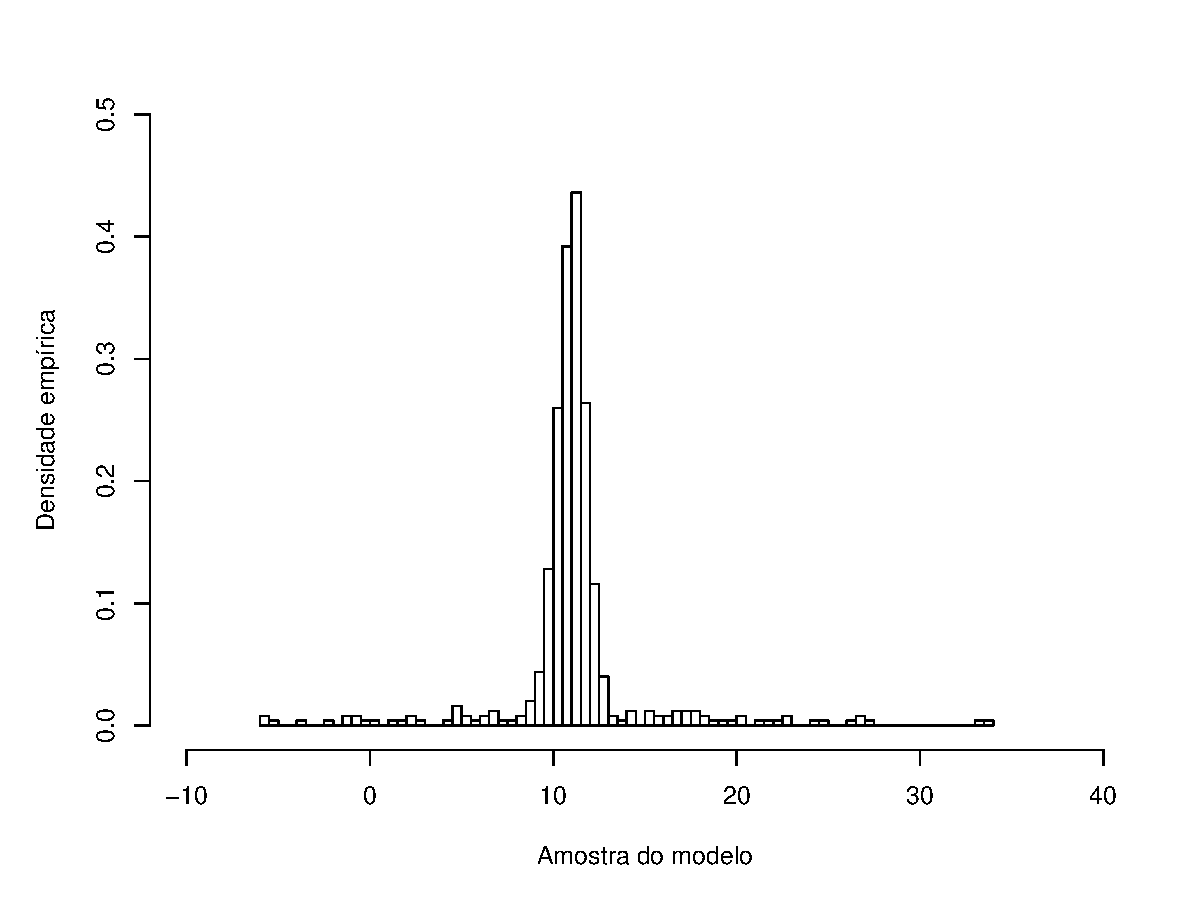
\includegraphics[scale=0.5]{amostra_n.pdf}
	\caption{Histograma da amostra gerada do modelo}
	\label{fig:sample_n.pdf}
\end{figure}
\end{frame}
% ==================================================
% ==================================================
\begin{frame}
\begin{figure}[htb]\footnotesize
	\centering
	\subfloat[$I_{\mu} = (10.85,11.13)$, dados $\sigma^2 = 0.64, \nu = 0.2$]{
		{
			\label{fig:maspro_mu}
			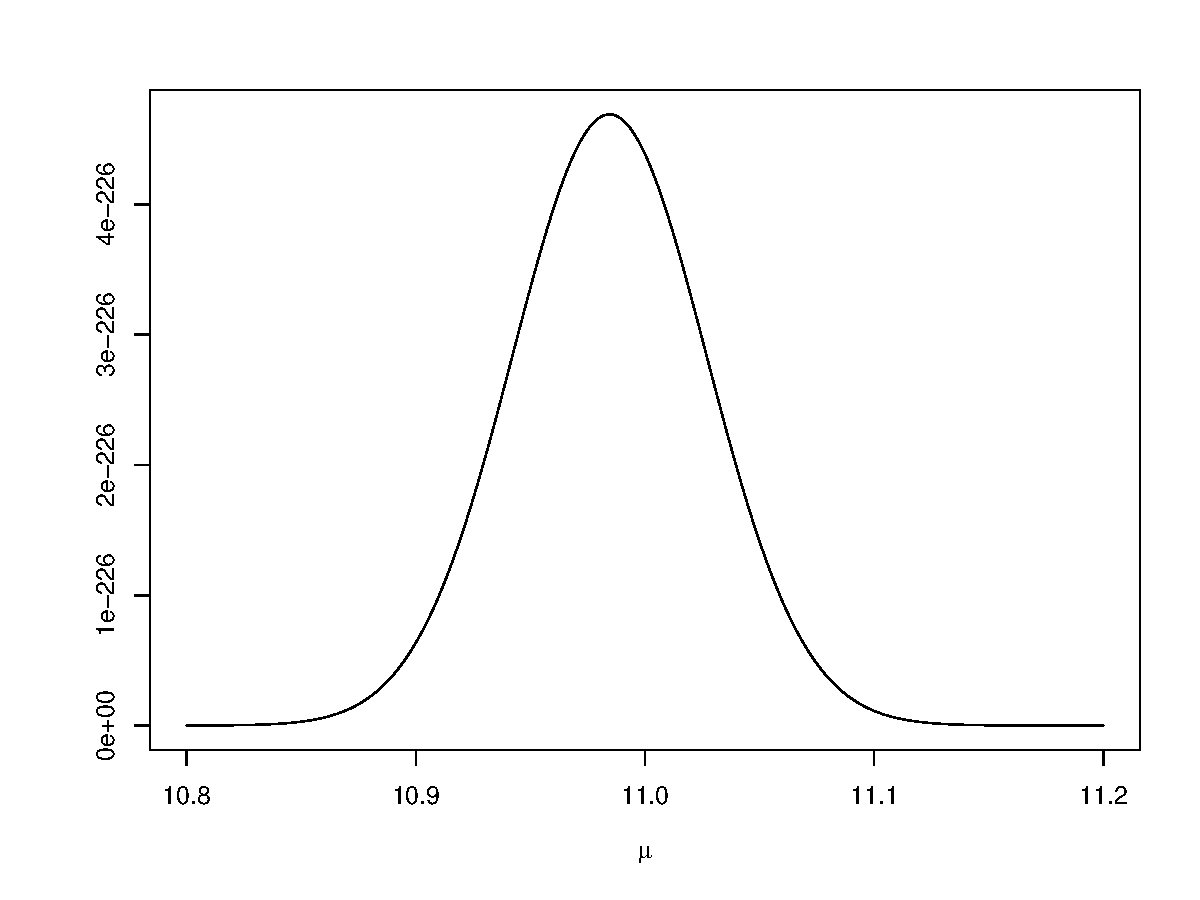
\includegraphics[scale=0.4]{maspro_mu.pdf}}}%
\caption{Intervalos de massa probabilística para cada parâmetro (variável aleatória) do núcleo de $p(\mu, \sigma^2, \nu | \bm{x})$}%
\end{figure}
\end{frame}
% ==================================================
% ==================================================
\begin{frame}
\begin{figure}[htb]\footnotesize
	\subfloat[$I_{\sigma^2} = (0.48, 0.78)$, dados $\mu = 11, \nu = 0.2$]{
	{
	\label{fig:maspro_s2}
		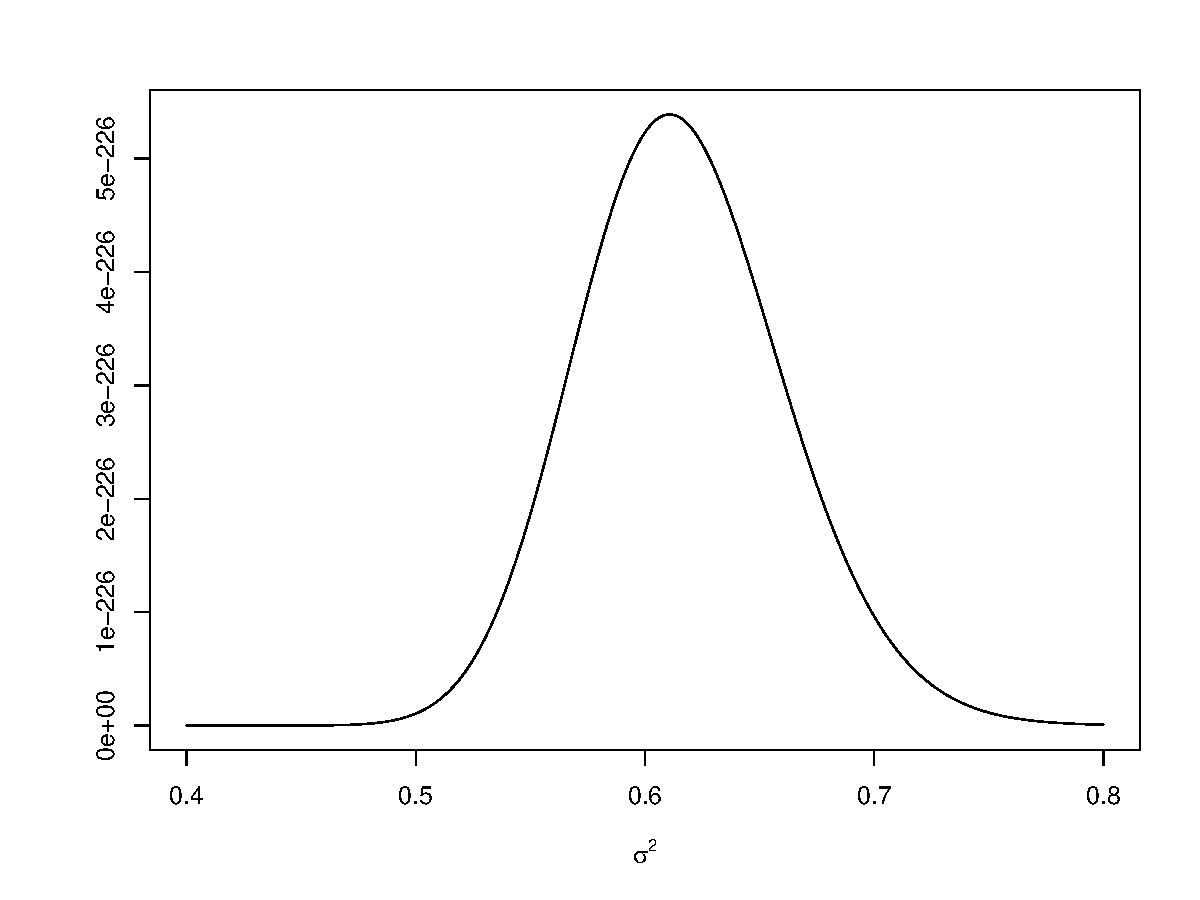
\includegraphics[scale=0.28]{maspro_s2.pdf}}}%
\subfloat[$I_{\nu} = (0.13, 0.26)$ dados $\mu = 11, \sigma^2 = 0.64$]{
	{
		\label{fig:maspro_nu}
		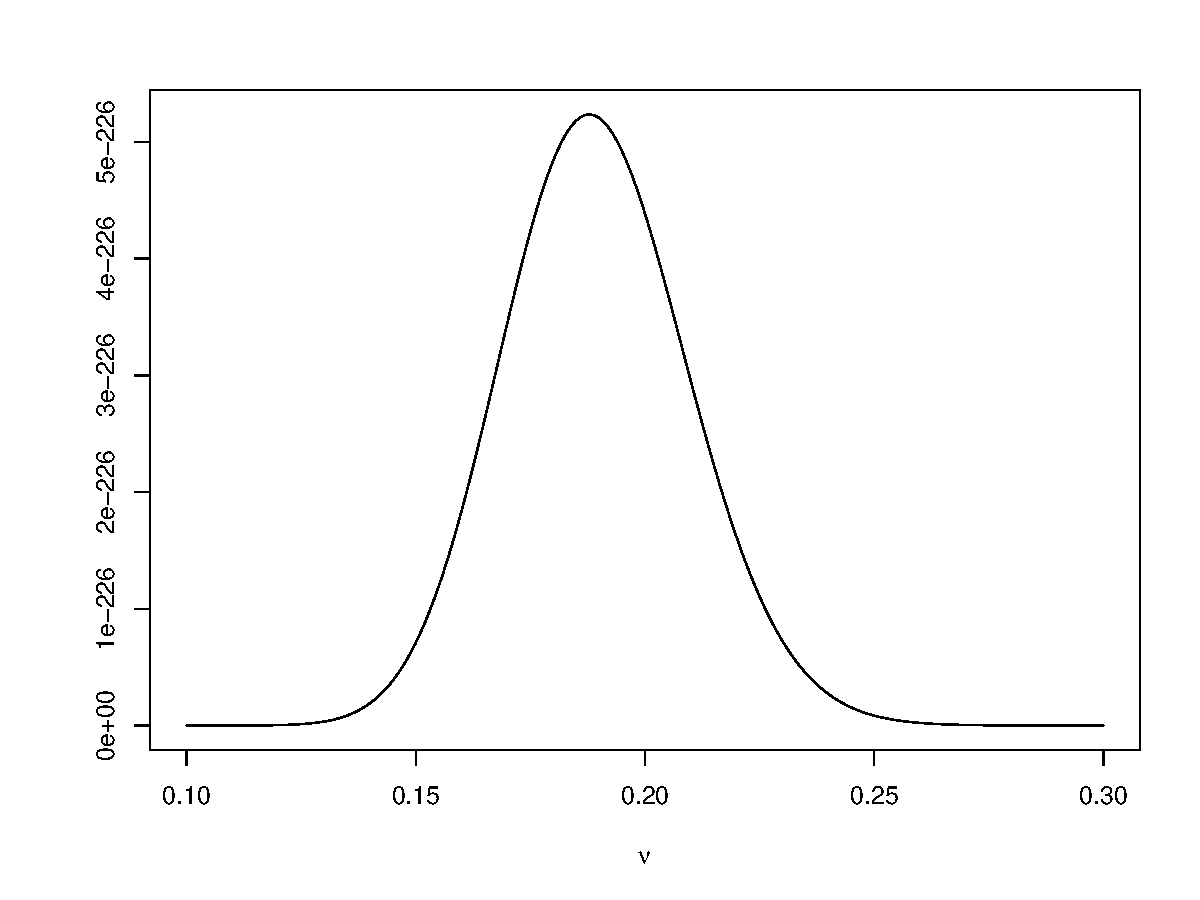
\includegraphics[scale=0.28]{maspro_nu.pdf}}}%
\caption{Intervalos de massa probabilística para cada parâmetro (variável aleatória) do núcleo de $p(\mu, \sigma^2, \nu | \bm{x})$}%
\end{figure}
\end{frame}
% ==================================================
% ==================================================
\section{Método de Quadratura de Riemann}
\begin{frame}
\begin{itemize}
\justifying	
\item Antes de aproximar as densidades \textit{a posteriori} marginais de cada parâmetro, é necessário aproximar o inverso da constante de proporcionalidade.
\item Dados três parâmetros $(\alpha_1, \alpha_2, \alpha_3)$ e uma amostra dos dados $\mathbf{y}$, quaisquer, suponha que se deseja aproximar a densidade \textit{a posteriori} marginal de $\alpha_3$ dados os pontos $r_i, s_j, t_k$ da grade formada por todos os subintervalos de integração, $i, j, k \in \{1, \ldots, L\}$. Temos pela quadratura de Riemann que
\begin{align}
p(\alpha_3 | \bm{y})
&= \iint p(\alpha_1, \alpha_2, \alpha_3 | \bm{y}) d\alpha_1 d\alpha_2 \nonumber \\
\Rightarrow p(t_k | \bm{y})
&= \iint p(\alpha_1, \alpha_2, t_k | \bm{y}) d\alpha_1 d\alpha_2 \approx \sum_{i=1}^{L} \sum_{j=1}^{L} p(r_i, s_j, t_k | \bm{y}) \Delta_i \Delta_j \nonumber \\
&= \sum_{i=1}^{L} \sum_{j=1}^{L} c \cdot h(r_i, s_j, t_k | \bm{y}) \Delta_i \Delta_j. \label{eq:dpm_riem}
\end{align}
\end{itemize}
\end{frame}
% ==================================================
% ==================================================
\begin{frame}
\begin{itemize}
\justifying	
\item Como $c$, a constante de proporcionalidade, é dada pelo inverso da densidade \textit{a priori} preditiva $f(\bm{y})$, a qual é obtida integrando-se em todo o espaço paramétrico o produto entre a função de verossimilhança $f(\bm{y} | \alpha_1, \alpha_2, \alpha_3)$ e as densidades (ou funções de probabilidade) \textit{a priori} para $\alpha_1$, $\alpha_2$ e $\alpha_3$, também é possível aproximar $c$ pela quadratura de Riemann
\item Neste caso, $c^{-1} \approx \sum_{i=1}^{L} \sum_{j=1}^{L} \sum_{k=1}^{L} h(r_i, s_j, t_k | \bm{y}) \Delta_i \Delta_j \Delta_k$. Com o valor aproximado para $c$, é possível calcular \eqref{eq:dpm_riem} nos limites superior e inferior de todos os subintervalos de um dado parâmetro e enfim obter uma aproximação da densidade \emph{a posteriori} marginal deste mesmo parâmetro através de uma curva gráfica que liga todos os valores calculados
\end{itemize}
\end{frame}
% ==================================================
% ==================================================
\begin{frame}
\begin{figure}[t]%
	\centering
	\subfloat[Densidade \textit{a posteriori} de $\mu$]{{
			\label{fig:dpm_mu_qr_15}
			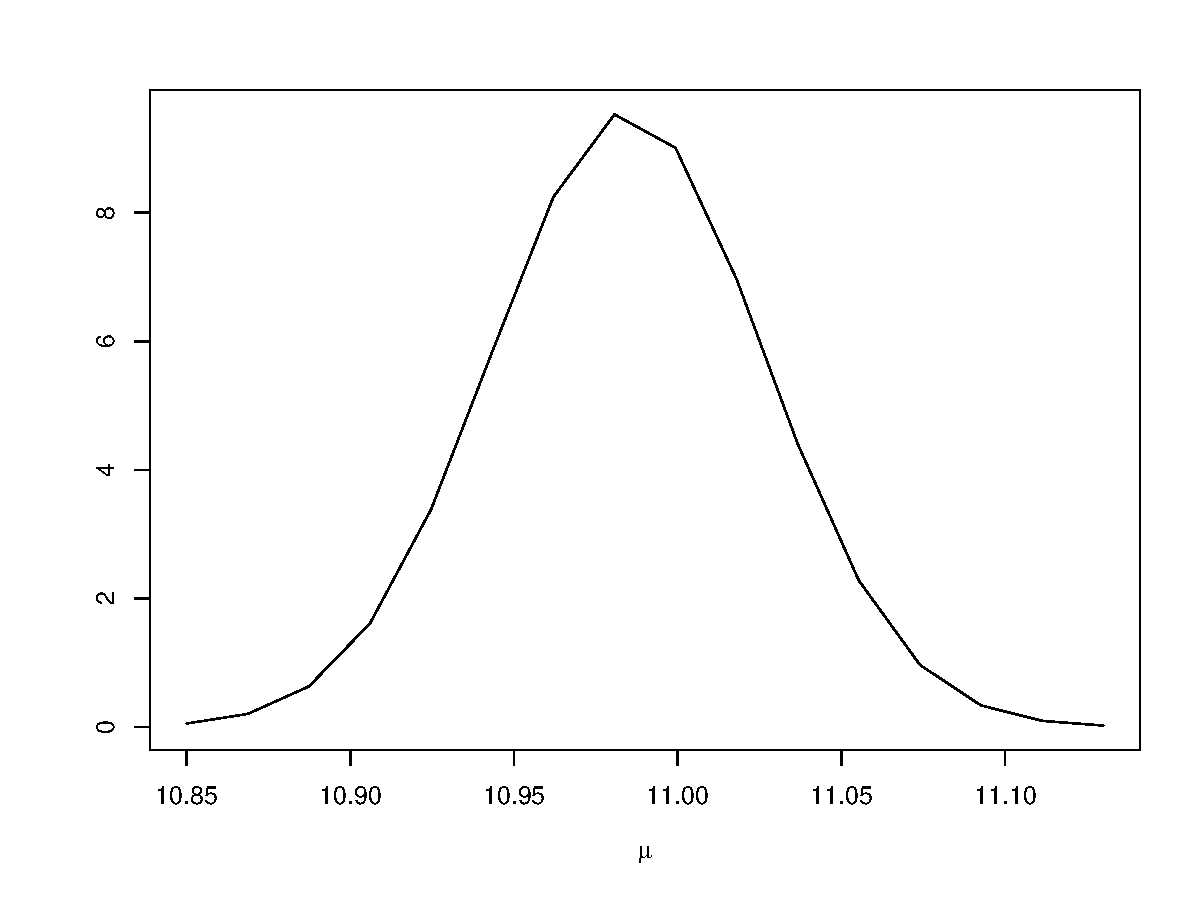
\includegraphics[scale=0.2]{dpm_mu_qr_15.pdf}}}%
	\qquad
	\subfloat[Densidade \textit{a posteriori} de $\sigma^2$]{{
			\label{fig:dpm_s2_qr_15}
			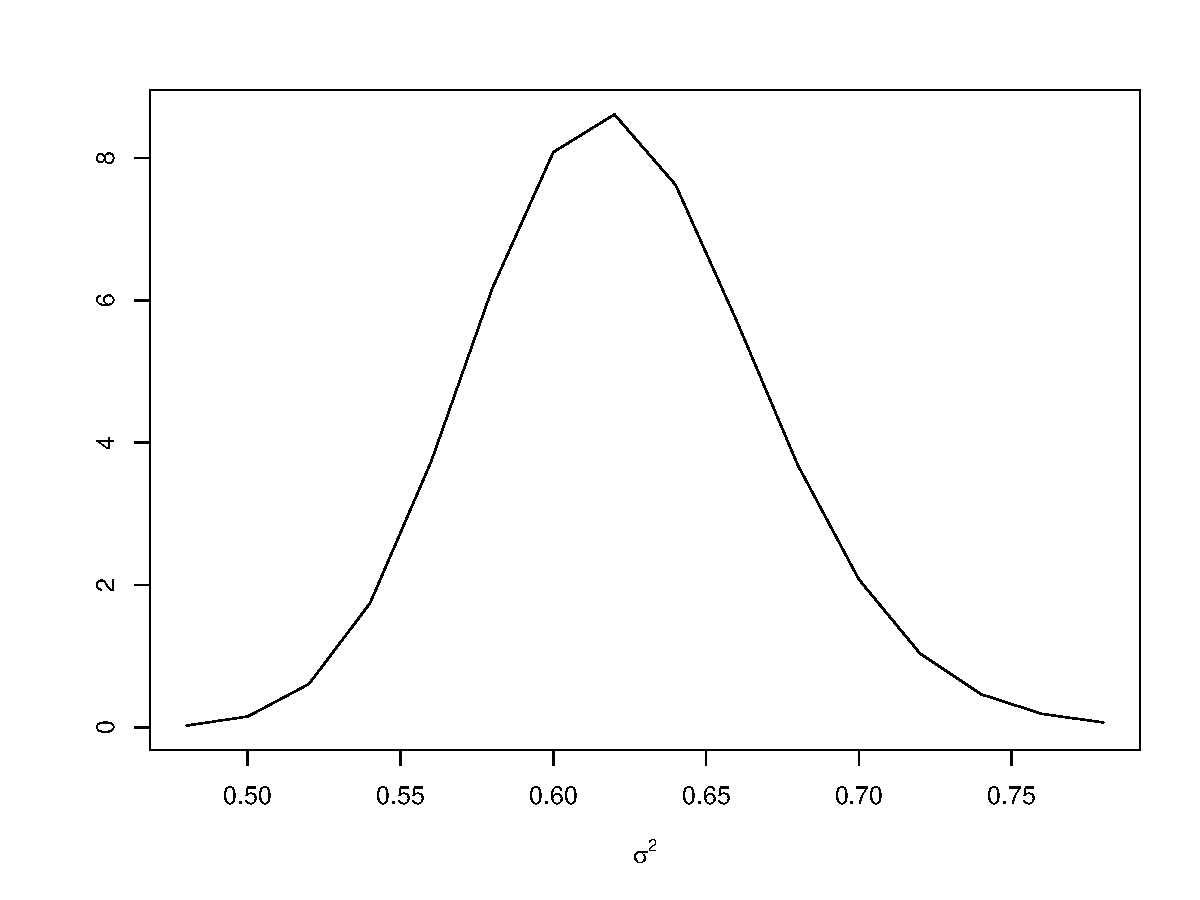
\includegraphics[scale=0.2]{dpm_s2_qr_15.pdf}}}%
	\subfloat[Densidade \textit{a posteriori} de $\nu$]{{
			\label{fig:dpm_nu_qr_15}
			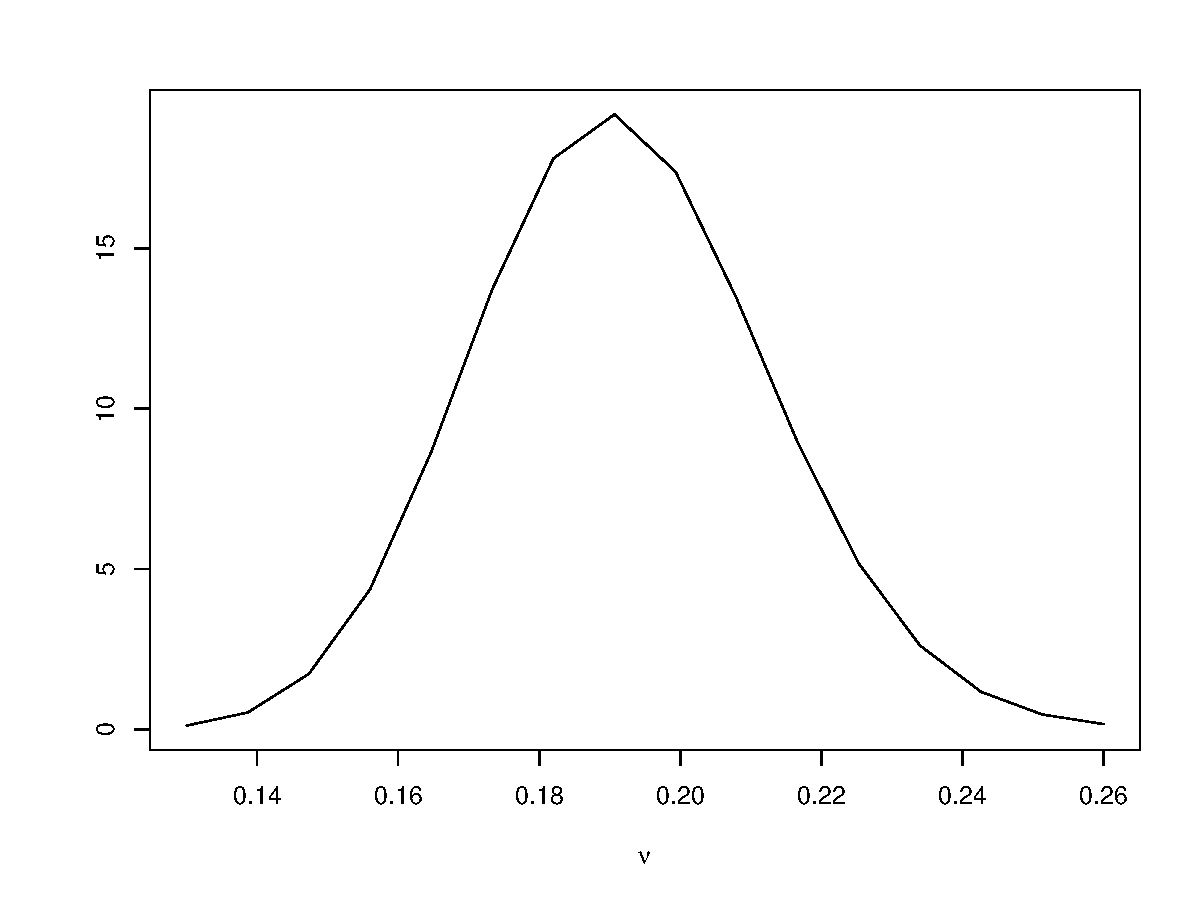
\includegraphics[scale=0.2]{dpm_nu_qr_15.pdf}}}%
	\caption{Densidades \textit{a posteriori} marginais pela quadratura de Riemann com $L = 15$}%
\end{figure}
\end{frame}
% ==================================================
% ==================================================
\begin{frame}
\begin{figure}[t]%
	\centering
	\subfloat[Densidade \textit{a posteriori} de $\mu$]{{
			\label{fig:dpm_mu_qr_50}
			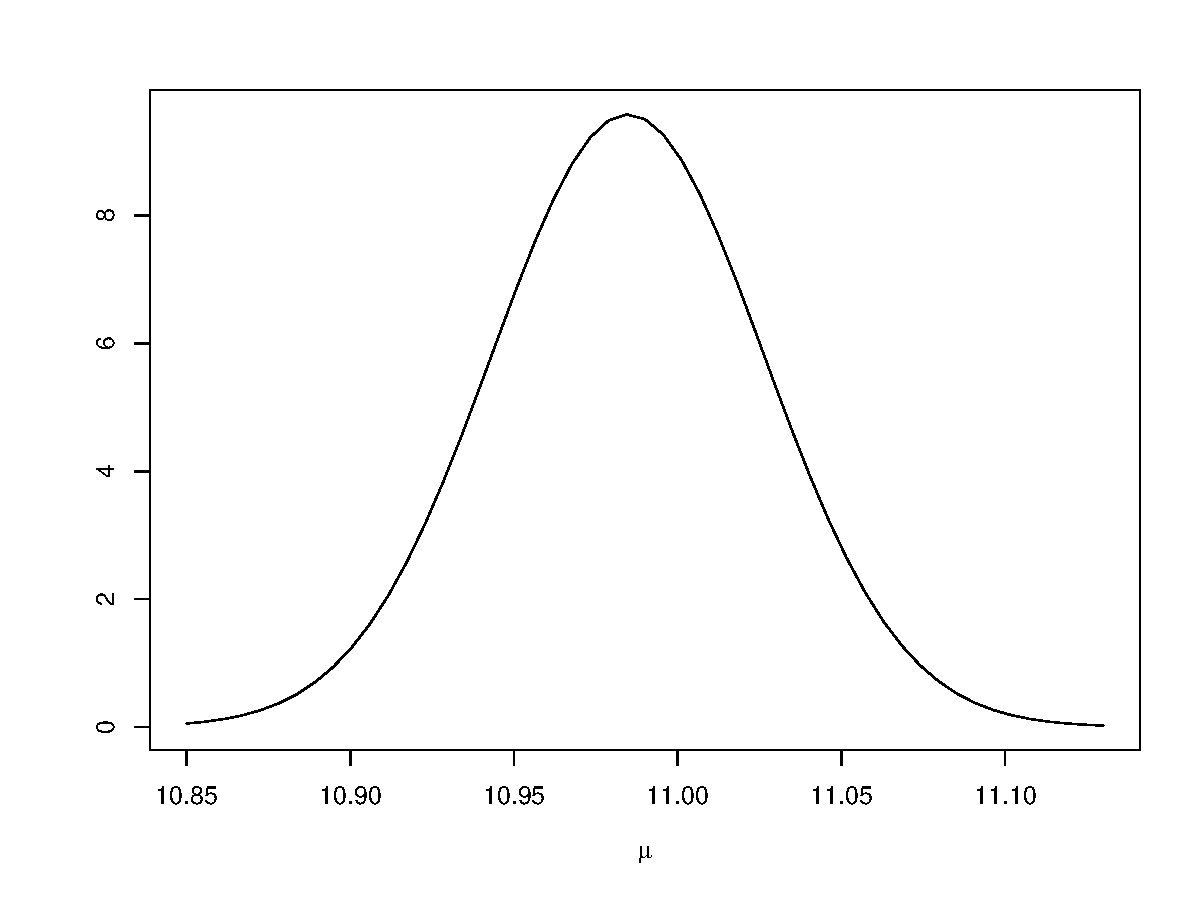
\includegraphics[scale=0.2]{dpm_mu_qr_50.pdf}}}%
	\qquad
	\subfloat[Densidade \textit{a posteriori} de $\sigma^2$]{{
			\label{fig:dpm_s2_qr_50}
			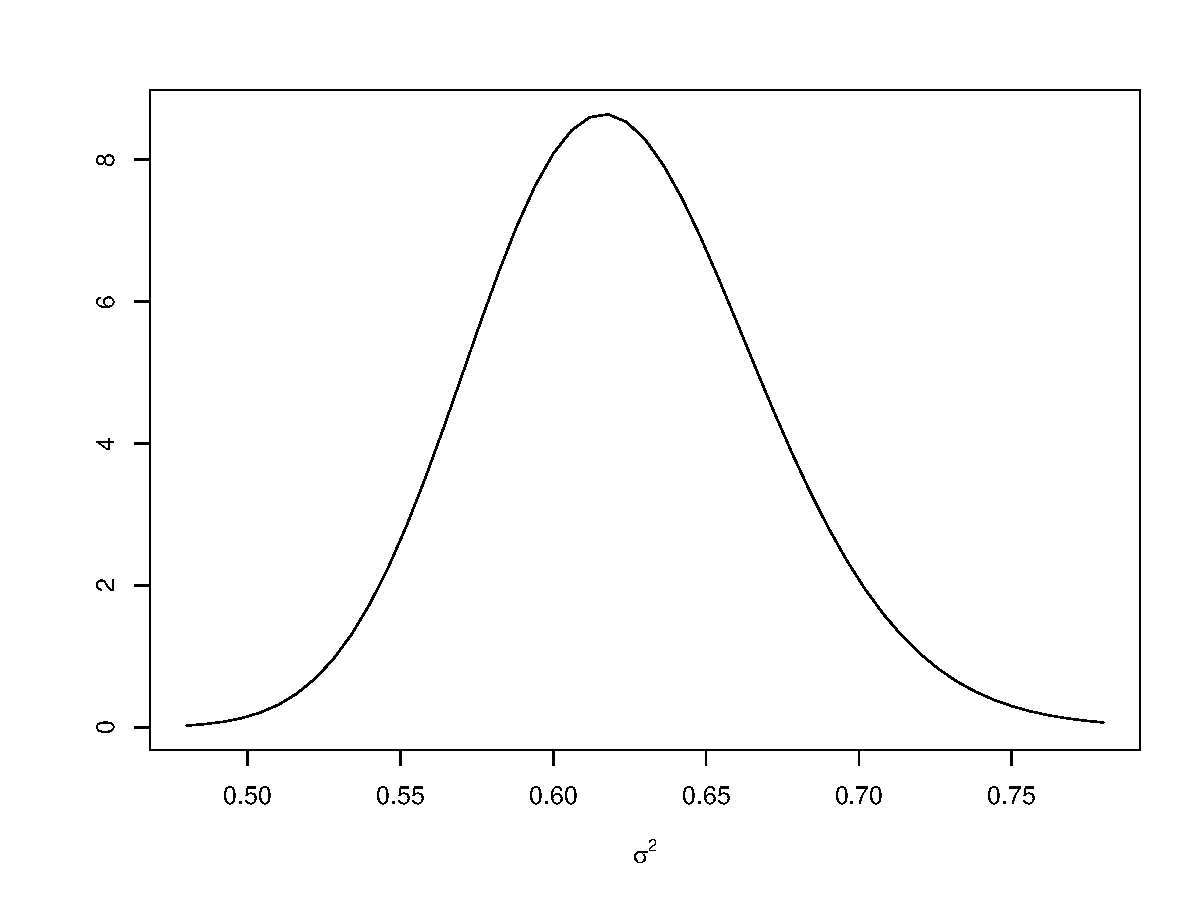
\includegraphics[scale=0.2]{dpm_s2_qr_50.pdf}}}%
	\subfloat[Densidade \textit{a posteriori} de $\nu$]{{
			\label{fig:dpm_nu_qr_50}
			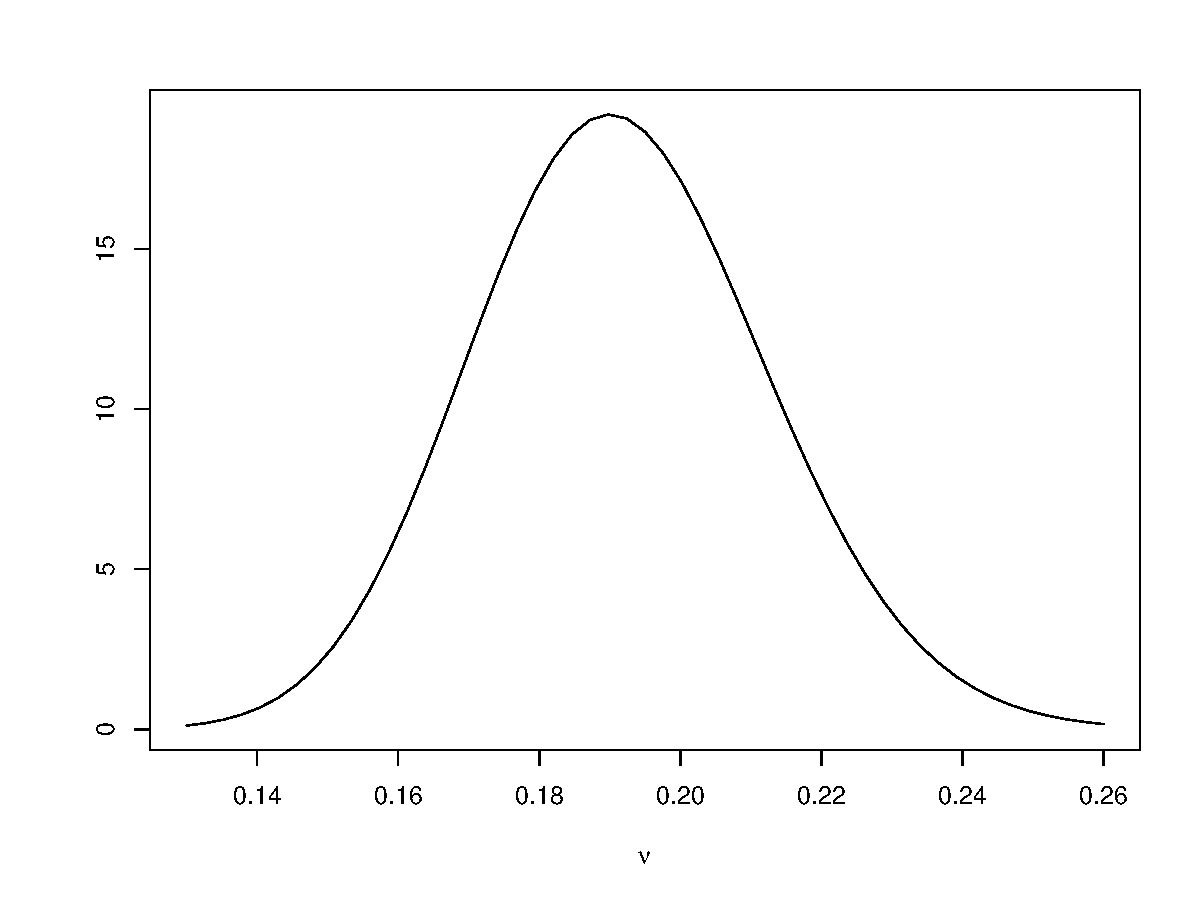
\includegraphics[scale=0.2]{dpm_nu_qr_50.pdf}}}%
	\caption{Densidades \textit{a posteriori} marginais pela quadratura de Riemann com $L = 50$}%
\end{figure}
\end{frame}
% ==================================================
% ==================================================
\begin{frame}
\begin{figure}[t]%
	\centering
	\subfloat[Densidade \textit{a posteriori} de $\mu$]{{
			\label{fig:dpm_mu_qr_100}
			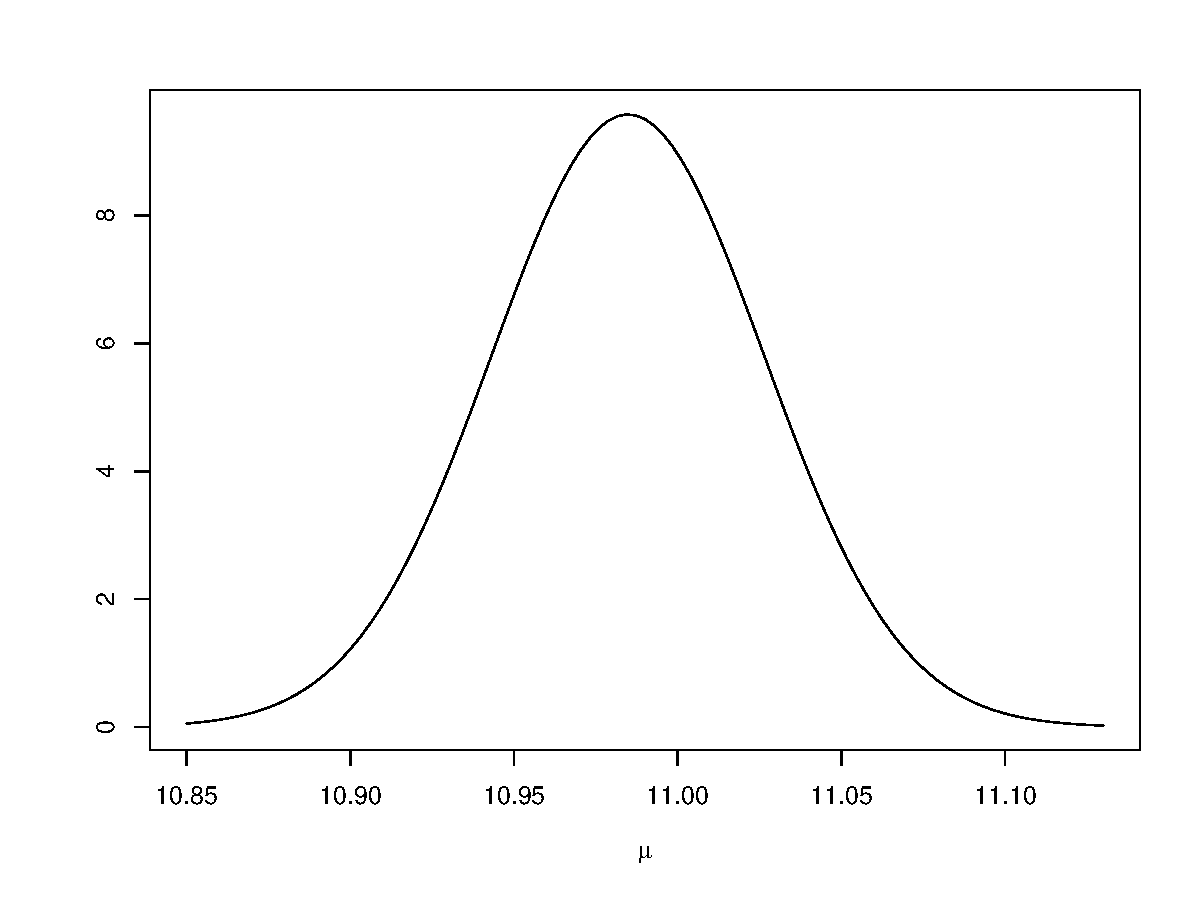
\includegraphics[scale=0.2]{dpm_mu_qr_100.pdf}}}%
	\qquad
	\subfloat[Densidade \textit{a posteriori} de $\sigma^2$]{{
			\label{fig:dpm_s2_qr_100}
			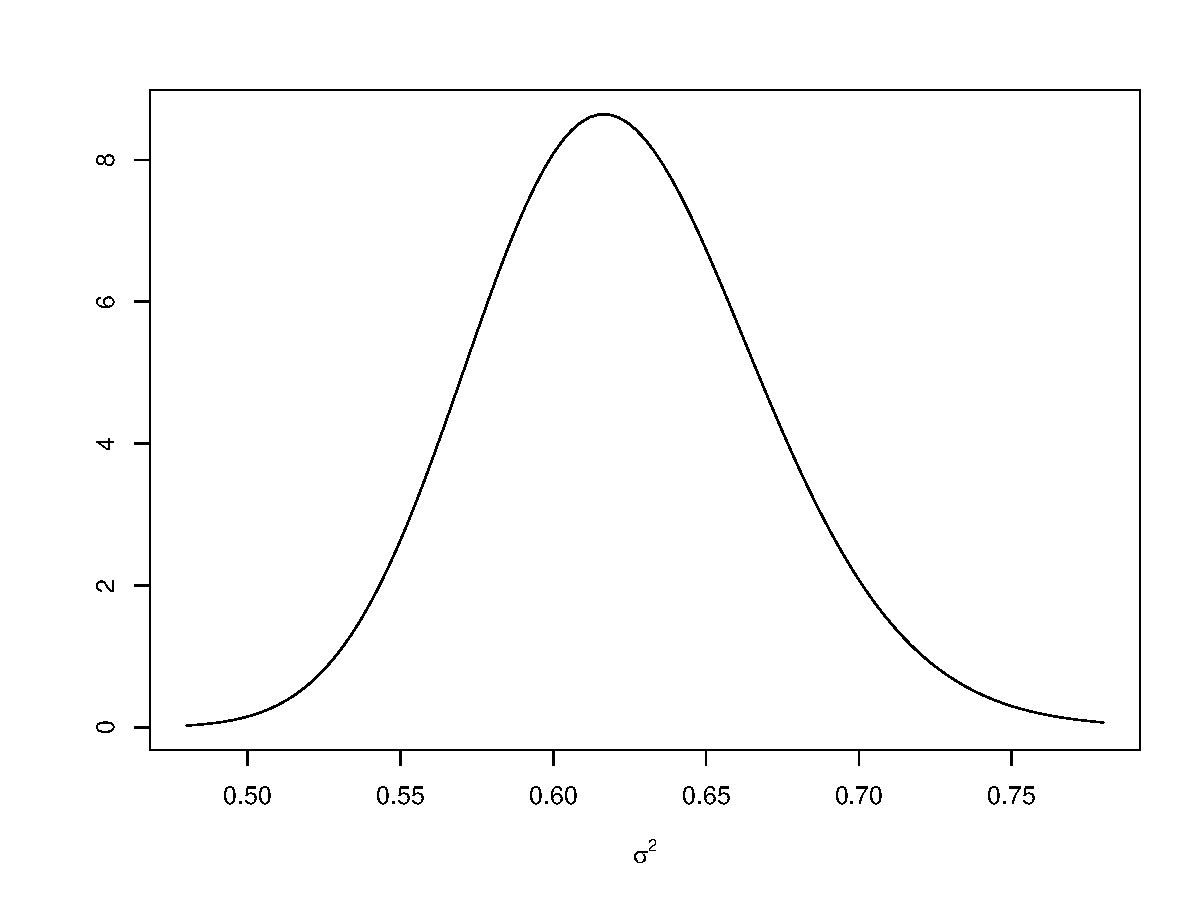
\includegraphics[scale=0.2]{dpm_s2_qr_100.pdf}}}%
	\subfloat[Densidade \textit{a posteriori} de $\nu$]{{
			\label{fig:dpm_nu_qr_100}
			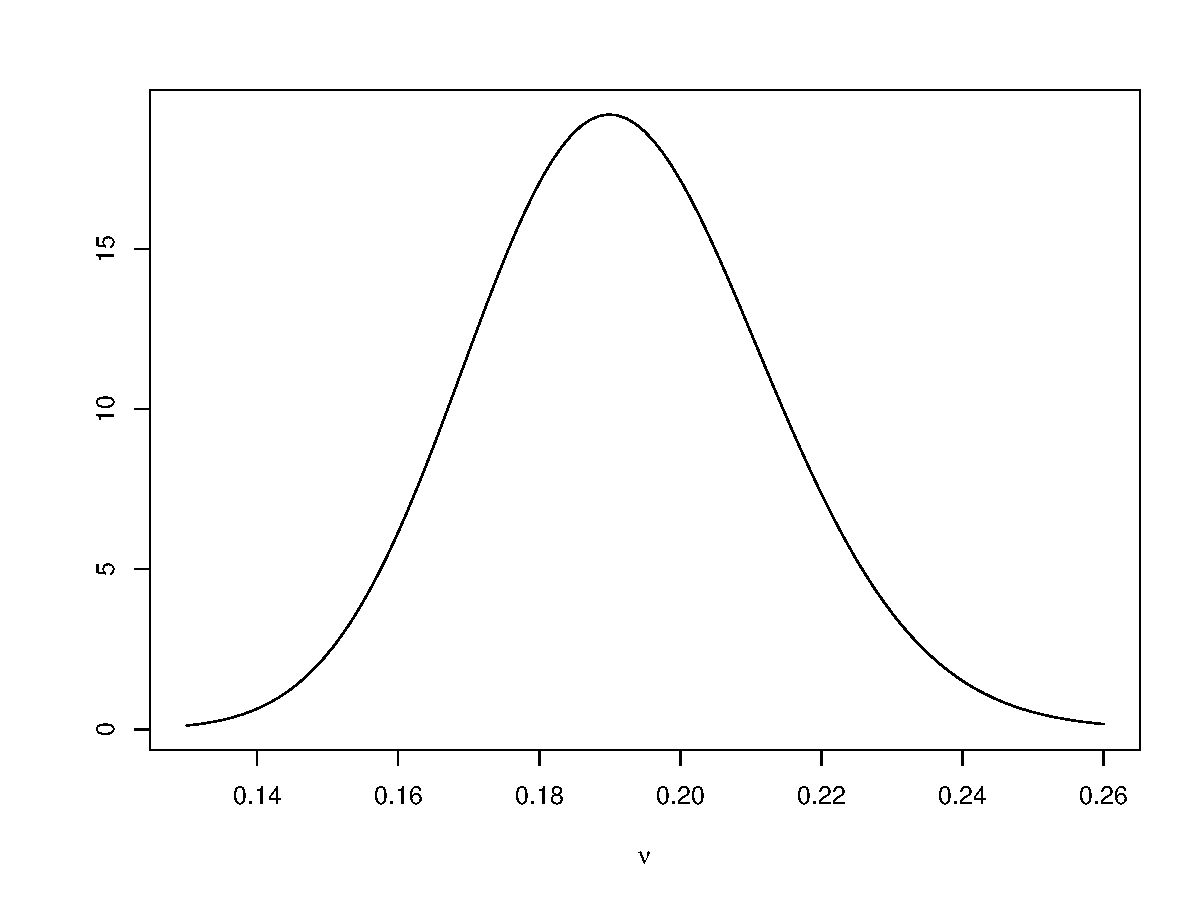
\includegraphics[scale=0.2]{dpm_nu_qr_100.pdf}}}%
	\caption{Densidades \textit{a posteriori} marginais pela quadratura de Riemann com $L = 100$}%
\end{figure}
\end{frame}
% ==================================================
% ==================================================
\begin{frame}
\begin{table}[htb]
	\caption{Estatísticas \textit{a posteriori} para $(\mu, \sigma^2, \nu)$ pela quadratura de Riemann}
	\label{tab1}
	\centering
	\begin{tabular}{cccccc}
		\toprule
		Cenário & Parâmetro & Média & Variância & Assimetria & Curtose \\
		\midrule
		$L = 15$ & $\mu$      & 10.9847 & 0.0017 & 0.0022 & 2.9603 \\
		& $\sigma^2$ &  0.6222 & 0.0022 & 0.2230 & 2.9984 \\
		& $\nu$      &  0.1918 & 0.0004 & 0.1572 & 2.9348 \\
		\midrule
		$L = 50$ & $\mu$      & 10.9848 & 0.0017 & 0.0056 & 2.9346 \\
		& $\sigma^2$ &  0.6222 & 0.0021 & 0.2149 & 2.9625 \\
		& $\nu$      &  0.1918 & 0.0004 & 0.1523 & 2.8995 \\
		\midrule
		$L = 100$ & $\mu$      & 10.9848 & 0.0017 & 0.0064 & 2.9284 \\
		& $\sigma^2$ &  0.6222 & 0.0021 & 0.2131 & 2.9542 \\
		& $\nu$      &  0.1918 & 0.0004 & 0.1512 & 2.8913 \\
		\bottomrule
	\end{tabular}
\end{table}
\end{frame}
% ==================================================
% ==================================================
\section{Reamostragem por importância sequêncial(SIR)}
\begin{frame}
\begin{itemize}
\justifying	
\item Proposto por Gordon \textit{et al.} (1993), o método SIR utiliza uma \textit{função de amostragem por importância} $g$ para aproximar (sem perda de generalidade) uma densidade de interesse $p$.

\item Sejam $\theta_1, \ldots, \theta_k$ uma amostra aleatória de $g$ e $\bm{y} = (y_1, \ldots, y_n)$ uma amostra do modelo para os dados observados. Para cada ponto $\theta_j$, $j = 1, \ldots, k$, os pesos são dados por
\begin{equation}\label{eq:sir_wei}
w_j(\theta_j) = \dfrac{p(\theta_j | \bm{y}) / q(\theta_j)}{\sum_{j=1}^{k} p(\theta_j | \bm{y}) / q(\theta_j)}.
\end{equation}
em que $g$  é uma densidade conhecida e da qual se sabe gerar uma amostra aleatória. 
\item Como feito em muitos trabalhos, para $g$ será escolhida uma densidade normal trivariada $N_3(\bm{\mu}, \bm{\Sigma})$, cujas componentes têm, cada uma, suporte em toda a reta real.
\end{itemize}
\end{frame}
% ==================================================
% ==================================================
\begin{frame}
\begin{itemize}
\justifying	
\item Note que para 2 parâmetros, $\sigma^2$ e $\nu$, o respectivo espaço paramétrico não é a reta real ($\Theta_{\sigma^2} = \mathbb{R}_+$ e $\Theta_{\nu} = [0,1]$, respectivamente). logo será feita uma reparametrização.
\item Para a reparametrização, consideram-se as transformações $\theta_1 = \mu, \theta_2 = \log(\sigma^2)$ e $\theta_3 = \log[\nu/(1-\nu)]$. Logo, a expressão do núcleo reparametrizado é dada por
\begin{align}
p(\theta_1, \theta_2, \theta_3 | \bm{x})
&= p(\theta_1 = \mu, \theta_2 = \log(\sigma^2), \theta_3 = \log[\nu/(1-\nu)] | \bm{x}) \nonumber \\
&= p(\mu = \theta_1, \sigma^2 = \exp(\theta_2), \nu = 1/[1 + \exp(-\theta_3)] | \bm{x}) \times |J(\theta_1, \theta_2, \theta_3)| \nonumber \\
&\propto \left[\exp(\theta_2)\right]^{-[(n + 1)/2 + a + 1]} \times \exp\left\{-\dfrac{\left[(\theta_1 - m)^2 / (2V) + d\right]}{\exp(\theta_2)}\right\} \nonumber \\
&\times A^*(\bm{x} | \theta_1, \theta_2, \theta_3) \times  \dfrac{\exp(\theta_2) \exp(\theta_3)}{\left[1 + \exp(-\theta_3)\right]^{-2}} \nonumber \\	&\propto \left(\dfrac{1}{\sigma^2}\right)^{\frac{n + 1}{2 + a + 1}} \times \exp\left\{-\dfrac{\left[(\mu - m)^2 / (2V) + d\right]}{\sigma^2}\right\} \times A(\bm{x} | \mu, \sigma^2, \nu) \nonumber \\
&\times \sigma^2 \nu^3(1-\nu)^{-1}, \label{eq:sir_dpre}
\end{align}
\end{itemize}
\end{frame}
% ==================================================
% ==================================================
\begin{frame}
\begin{itemize}
\justifying	
\item em que $|J(\theta_1, \theta_2, \theta_3)|$ é o determinante da matriz jacobiana das derivadas parciais de $(\mu, \sigma^2, \nu)$ com respeito a $(\theta_1, \theta_2, \theta_3)$.
\item Para a amostra de tamanho $n=500$ da mistura finita de normais com variância contaminada tal que $\mu = 11$; $\sigma^2 = 0.64$; $\nu = 0.2$; $m = 11$; $V = 1$; $a = 7$ e $d = 4$ (Figura \ref{fig:sample_n.pdf}).

\item Para as médias das componentes desta distribuição, será fixado $\bm{\mu} = (\theta_1, \theta_2, \theta_3) = (\mu, \log(\sigma^2), \log[\nu/(1-\nu)]) = (11, \log(0.64), \log[0.2/0.8])$.
\item Para a matriz de covariância $\bm{\Sigma}$, cada elemento da diagonal principal será dado pelo quadrado de $1/6$ do intervalo de massa probabilística do parâmetro correspondente.

\item Esta escolha se justifica pelo fato de que as distribuições mostradas de \ref{fig:maspro_mu} a \ref{fig:maspro_nu} têm comportamento próximo à normalidade.
\end{itemize}
\end{frame}
% ==================================================
% ==================================================
\begin{frame}
\begin{figure}[t]%
	\centering
	\subfloat[Histograma de $\mu$]{{
			\label{fig:mu_sir_500}
			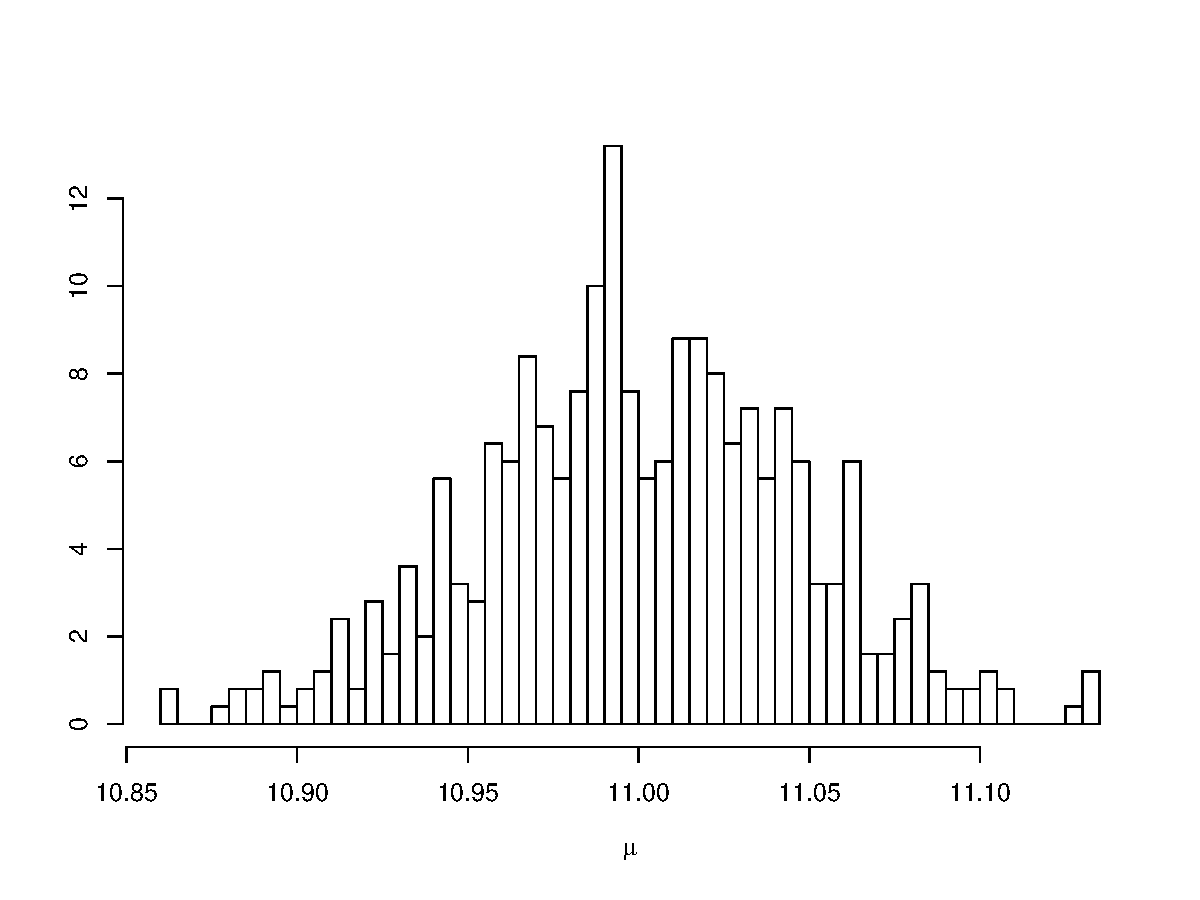
\includegraphics[scale=0.2]{mu_sir_500.pdf}}}%
	\qquad
	\subfloat[Histograma de $\sigma^2$]{{
			\label{fig:s2_sir_500}
			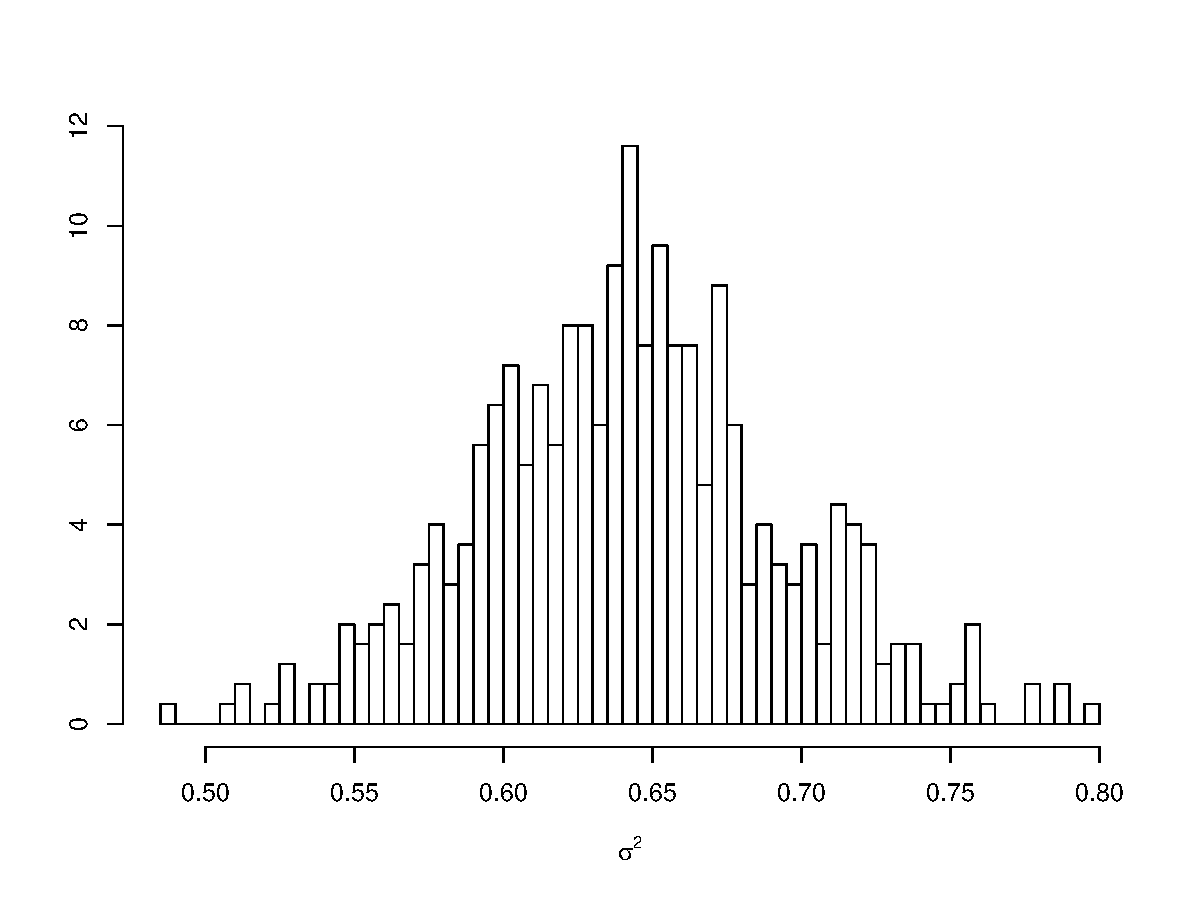
\includegraphics[scale=0.2]{s2_sir_500.pdf}}}%
	\subfloat[Histograma de $\nu$]{{
			\label{fig:nu_sir_500}
			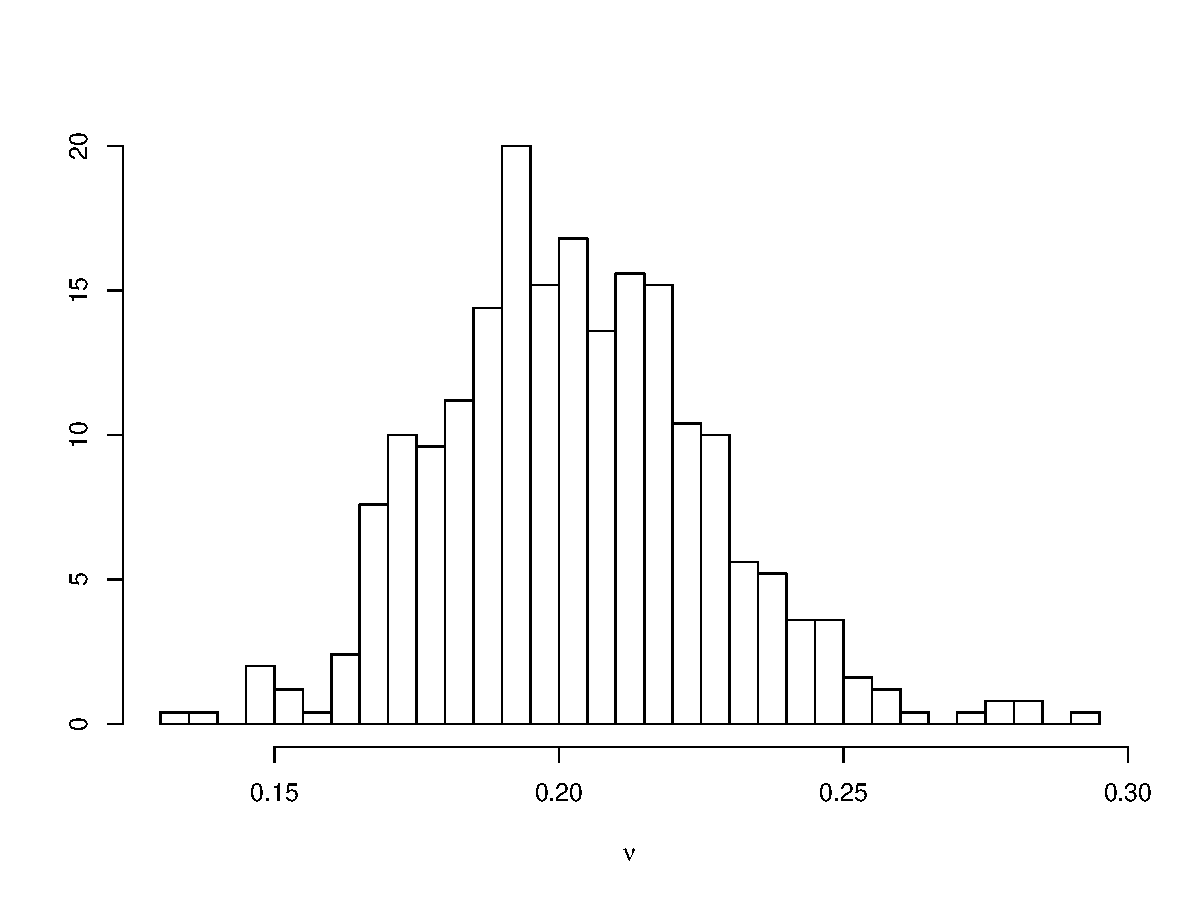
\includegraphics[scale=0.2]{nu_sir_500.pdf}}}%
	\caption{Histograma das densidades \textit{a posteriori} marginais pela método SIR com $k = 500$}%
\end{figure}
\end{frame}
% ==================================================
% ==================================================
\begin{frame}
\begin{figure}[t]%
	\centering
	\subfloat[Histograma de $\mu$]{{
			\label{fig:mu_sir_5000}
			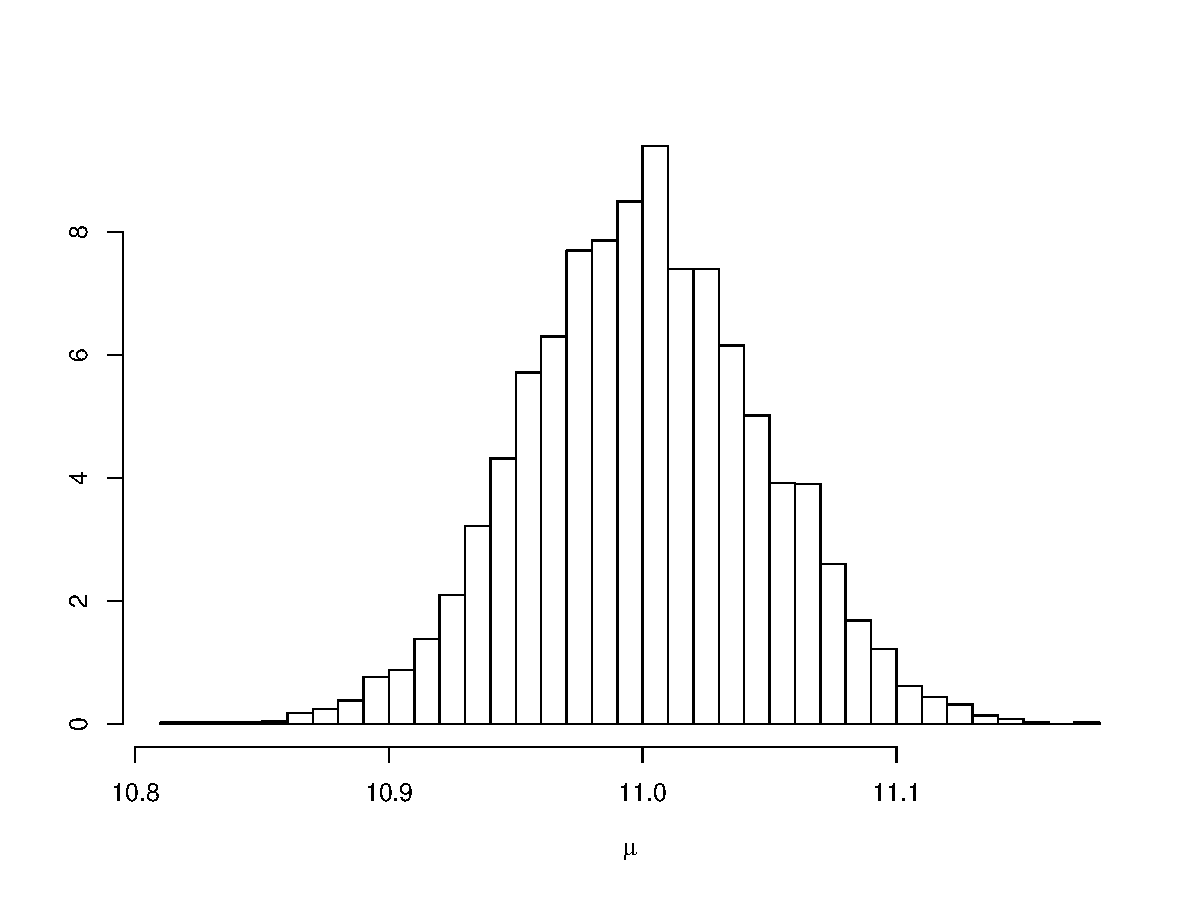
\includegraphics[scale=0.2]{mu_sir_5000.pdf}}}%
	\qquad
	\subfloat[Histograma de $\sigma^2$]{{
			\label{fig:s2_sir_5000}
			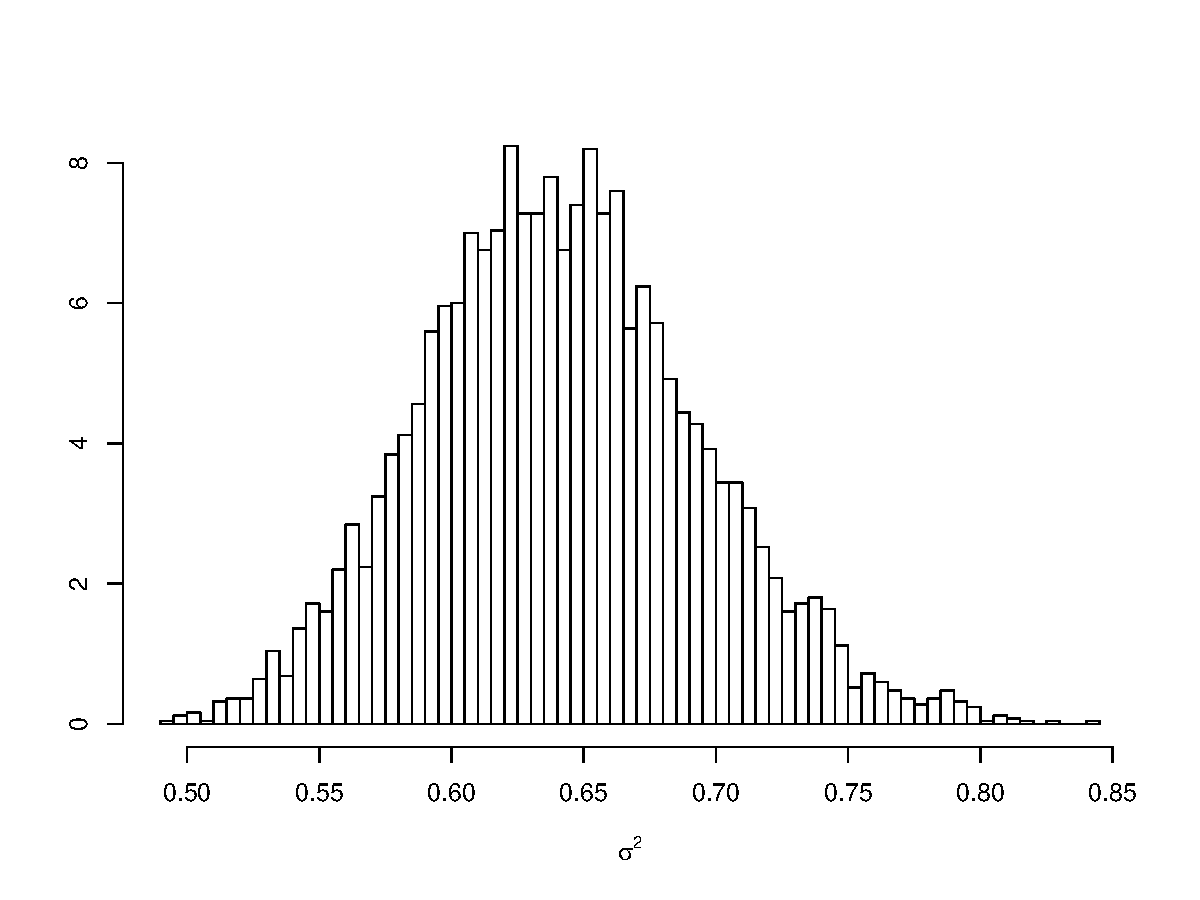
\includegraphics[scale=0.2]{s2_sir_5000.pdf}}}%
	\subfloat[Histograma de $\nu$]{{
			\label{fig:nu_sir_5000}
			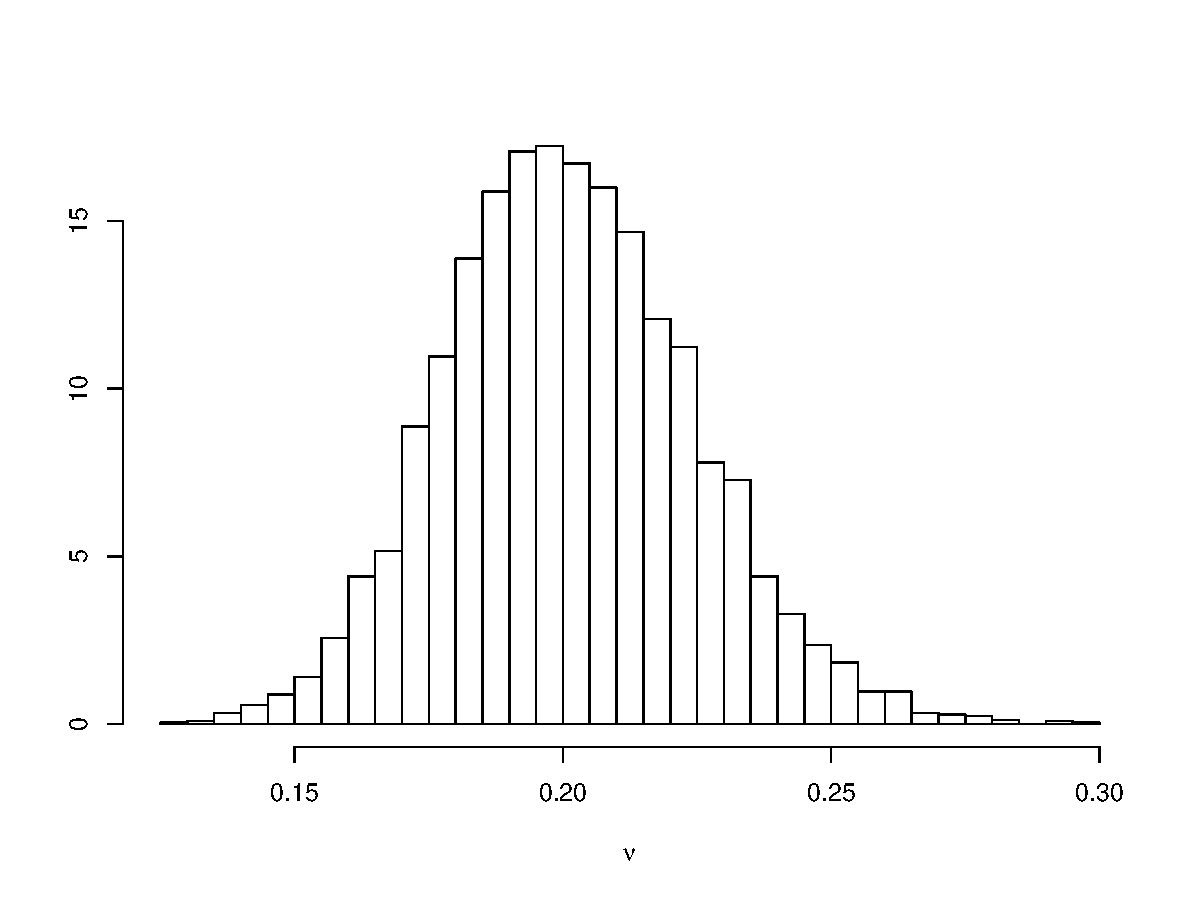
\includegraphics[scale=0.2]{nu_sir_5000.pdf}}}%
	\caption{Histograma das densidades \textit{a posteriori} marginais pela método SIR com $k = 5000$}%
\end{figure}
\end{frame}
% ==================================================
% ==================================================
\begin{frame}
\begin{figure}[t]%
	\centering
	\subfloat[Histograma de $\mu$]{{
			\label{fig:mu_sir_50000}
			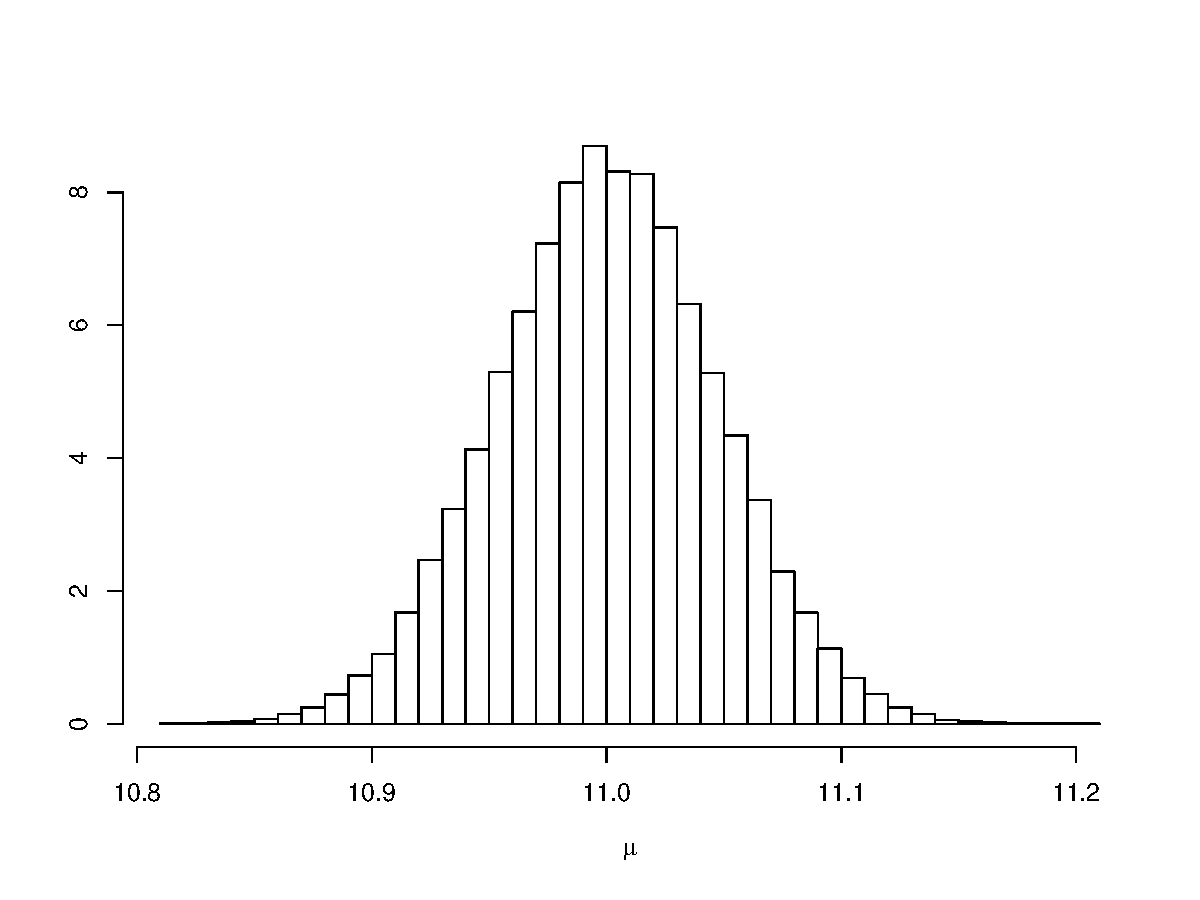
\includegraphics[scale=0.2]{mu_sir_50000.pdf}}}%
	\qquad
	\subfloat[Histograma de $\sigma^2$]{{
			\label{fig:s2_sir_50000}
			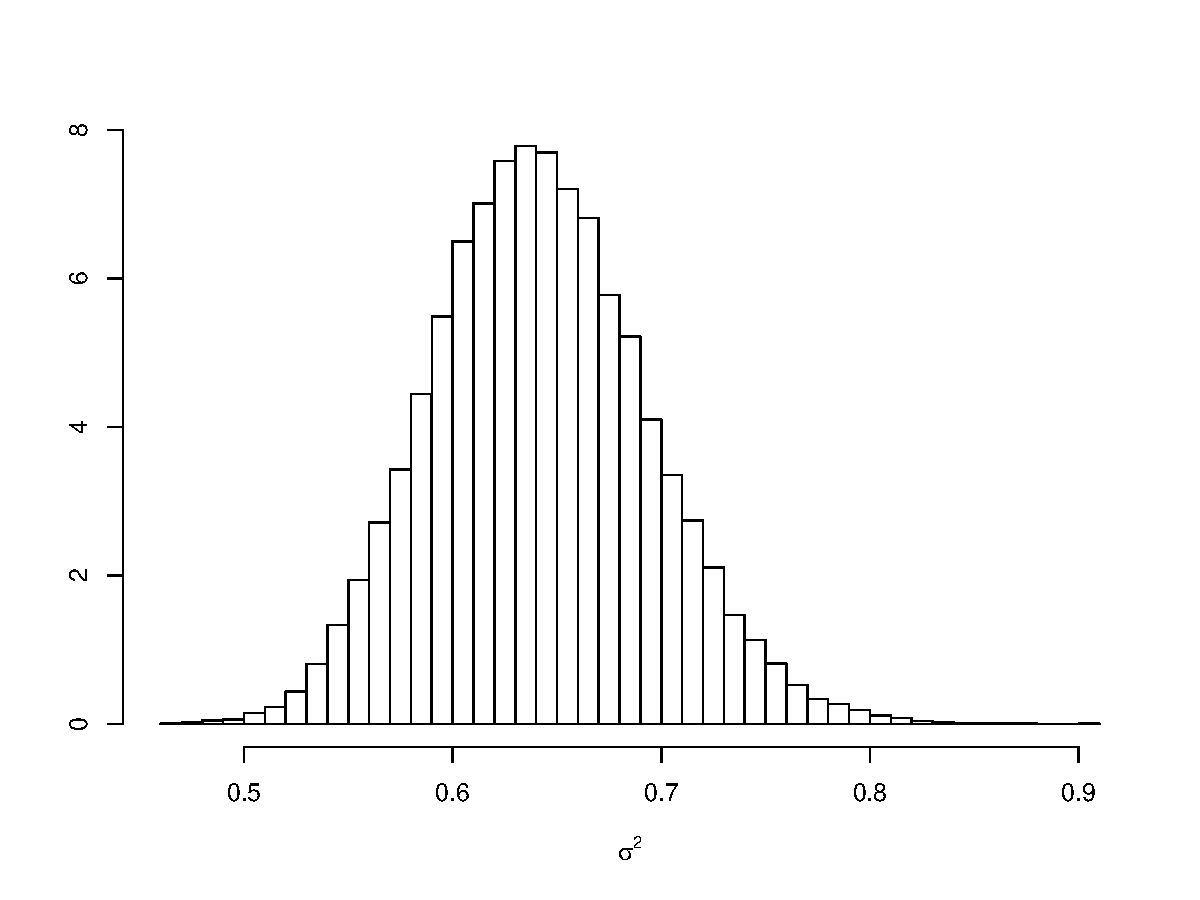
\includegraphics[scale=0.2]{s2_sir_50000.pdf}}}%
	\subfloat[Histograma de $\nu$]{{
			\label{fig:nu_sir_50000}
			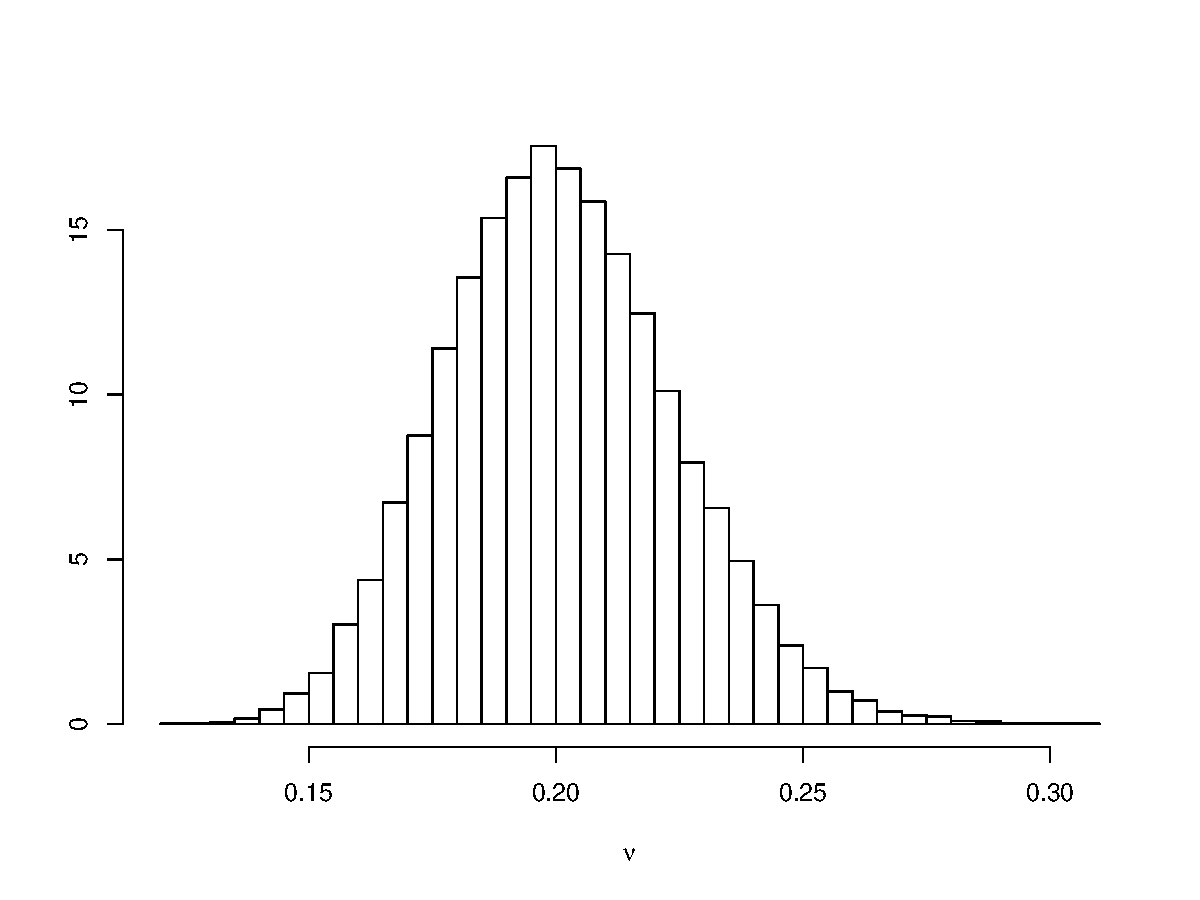
\includegraphics[scale=0.2]{nu_sir_50000.pdf}}}%
	\caption{Histograma das densidades \textit{a posteriori} marginais pela método SIR com $k = 50000$}%
\end{figure}
\end{frame}
% ==================================================
% ==================================================
\begin{frame}
\begin{table}[htb]
	\caption{Estatísticas \textit{a posteriori} para $(\mu, \sigma^2, \nu)$ pelo método SIR}
	\label{tab2}
	\centering
	\begin{tabular}{cccccc}
		\toprule
		Cenário & Parâmetro & Média & Variância & Assimetria & Curtose \\
		\midrule
		$k = 500$ & $\mu$      & 11.0003 & 0.0023 & -0.0610 & 3.0351 \\
		& $\sigma^2$ &  0.6422 & 0.0026 &  0.1261 & 3.1453 \\
		& $\nu$      &  0.2028 & 0.0006 &  0.3510 & 3.5475 \\
		\midrule
		$k = 5000$ & $\mu$      & 11.0006 & 0.0022 &  0.0216 & 3.0234 \\
		& $\sigma^2$ &  0.6418 & 0.0027 &  0.2349 & 3.0118 \\
		& $\nu$      &  0.2013 & 0.0005 &  0.2485 & 3.1646 \\
		\midrule
		$k = 50000$ & $\mu$      & 11.0002 & 0.0022 & -0.0081 & 3.0451 \\
		& $\sigma^2$ &  0.6420 & 0.0027 &  0.2353 & 3.1153 \\
		& $\nu$      &  0.2009 & 0.0005 &  0.2608 & 3.0849 \\
		\bottomrule
	\end{tabular}
\end{table}
\end{frame}
% ==================================================
% ==================================================
\section{Integração via Monte Carlo em cadeias de Markov}
% ==================================================
% ==================================================
\begin{frame}
\begin{itemize}
\justifying	
\item Neste trabalho, será usado o algoritmo de Metropolis-Hastings (Metropolis \textit{et al.}, 1953; Hastings, 1970), aqui abreviado por MH.
\item Assim como o método SIR, o algoritmo MH também é baseado no uso de uma distribuição auxiliar ou proposta, aqui denotada por $q(\bm{y}, \bm{z})$. Assumindo-se que na interação $j$, $j = 1, \ldots, k$ a cadeia está no estado $\bm{y}^{(j)}$, a posição da mesma na iteração $j + 1$, denotada por $\bm{y}^{(j + 1)}$, será dada após:
\item Passo 1: Propor uma transição ou movimento para $\bm{y}^*$, onde $\bm{y}^*$ é gerada de $q(\bm{y}^{(j)}, \cdot)$, a distribuição proposta, e, o valor inicial $\mathbf{y}^{(1)}$;
\item Passo 2: Aceitar a transição proposta com probabilidade
\begin{equation}\label{eq:mh_tranprob}
\rho(\bm{y}^{(j)}, \bm{y}^*) = \min\left(1, \dfrac{p(\bm{y}^*) / q(\bm{y}^{(j)}, \bm{y}^*)}{p(\bm{y}^{(j)}) / q(\bm{y}^*, \bm{y}^{(j)})}\right)
\end{equation}
e neste caso atribuir $\bm{y}^{(j + 1)} = \bm{y}^*$ ou rejeitar a transição proposta e atribuir $\bm{y}^{(j + 1)} = \bm{y}^{(j)}$, com probabilidade $1 - \rho(\bm{y}^{(j)}, \bm{y}^*)$.
\end{itemize}
\end{frame}
% ==================================================
% ==================================================
\begin{frame}
\begin{itemize}
\justifying	
\item Para decidir sobre a aceitação ou não de $\bm{y}^*$ quando amostrada a cada passo $j$, gere uma amostra $u_1, \ldots, u_k$, onde $k$ é o total de iterações prefixadas, da distribuição uniforme padrão $U(0,1)$, independentemente de $\bm{y}^*$.
\item Se a probabilidade de aceitação $\rho(\bm{y}^{(j)}, \bm{y}^*)$ for maior do que ou igual a $u_j$, então a transição proposta é aceita. Do contrário, ela é rejeitada.
\item Para a distribuição proposta $q(\cdot)$ também será escolhida uma normal trivariada $N_3(\bm{\mu}, \bm{\Sigma})$, com valores do vetor de médias, e será reutilizado a reparametrização $\bm{\mu} = (\mu, \log(\sigma^2), \log[\nu/(1-\nu)]) = (11, \log(0.64), \log[0.2/0.8])$ e da matriz de covariância $\bm{\Sigma} = \textrm{diag}\{0.0022, 0.0065, 0.0203\}$.
\item É necessário definir um estado inicial da cadeia, em geral com densidade conjunta muito baixa, escolheu-se o ponto $y^{(1)} = (10.86, \log(0.50),\log(0.14/0.86))$. 
\end{itemize}
\end{frame}
% ==================================================
% ==================================================
\begin{frame}
\begin{figure}[t]%
	\centering
	\subfloat[Histograma de $\mu$]{{
			\label{fig:mu_mh_500}
			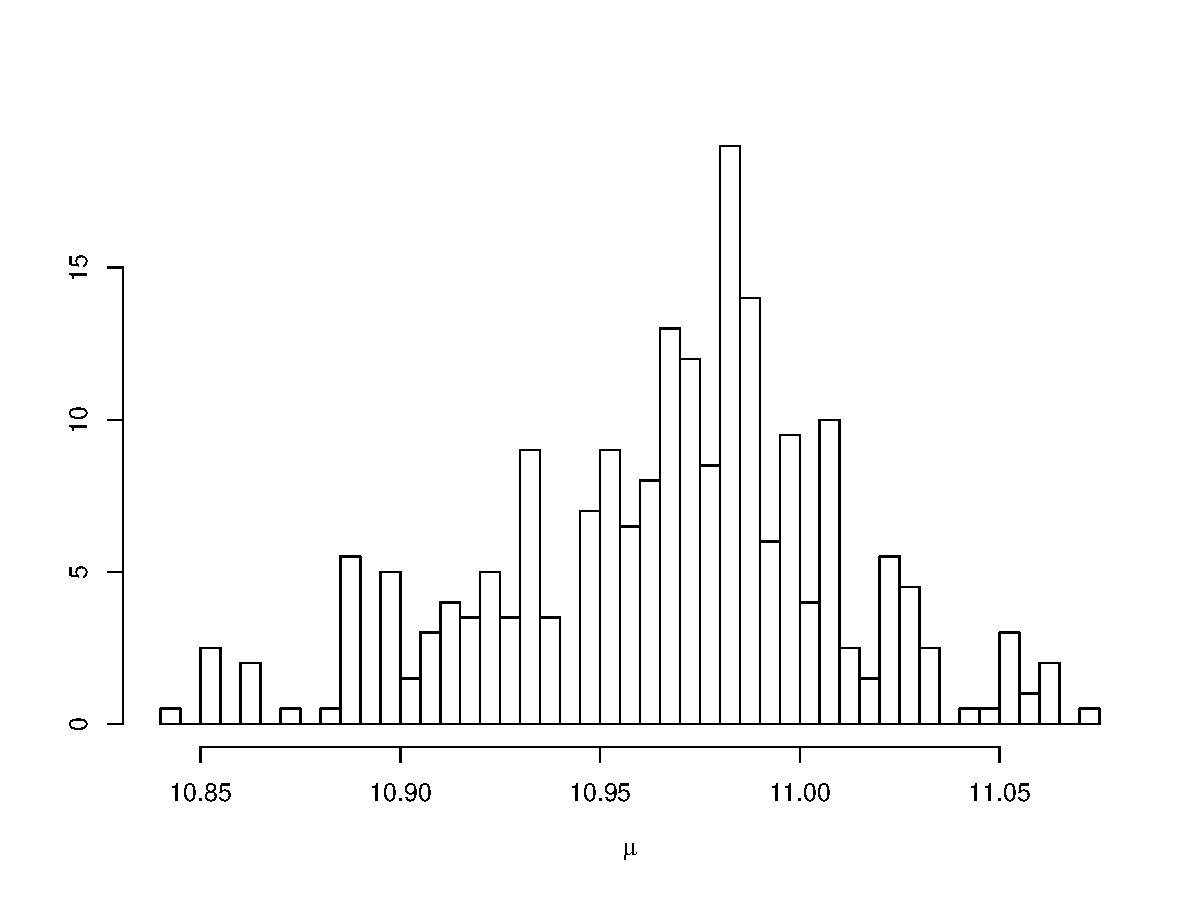
\includegraphics[scale=0.2]{mu_mh_500.pdf}}}%
	\qquad
	\subfloat[Histograma de $\sigma^2$]{{
			\label{fig:s2_mh_500}
			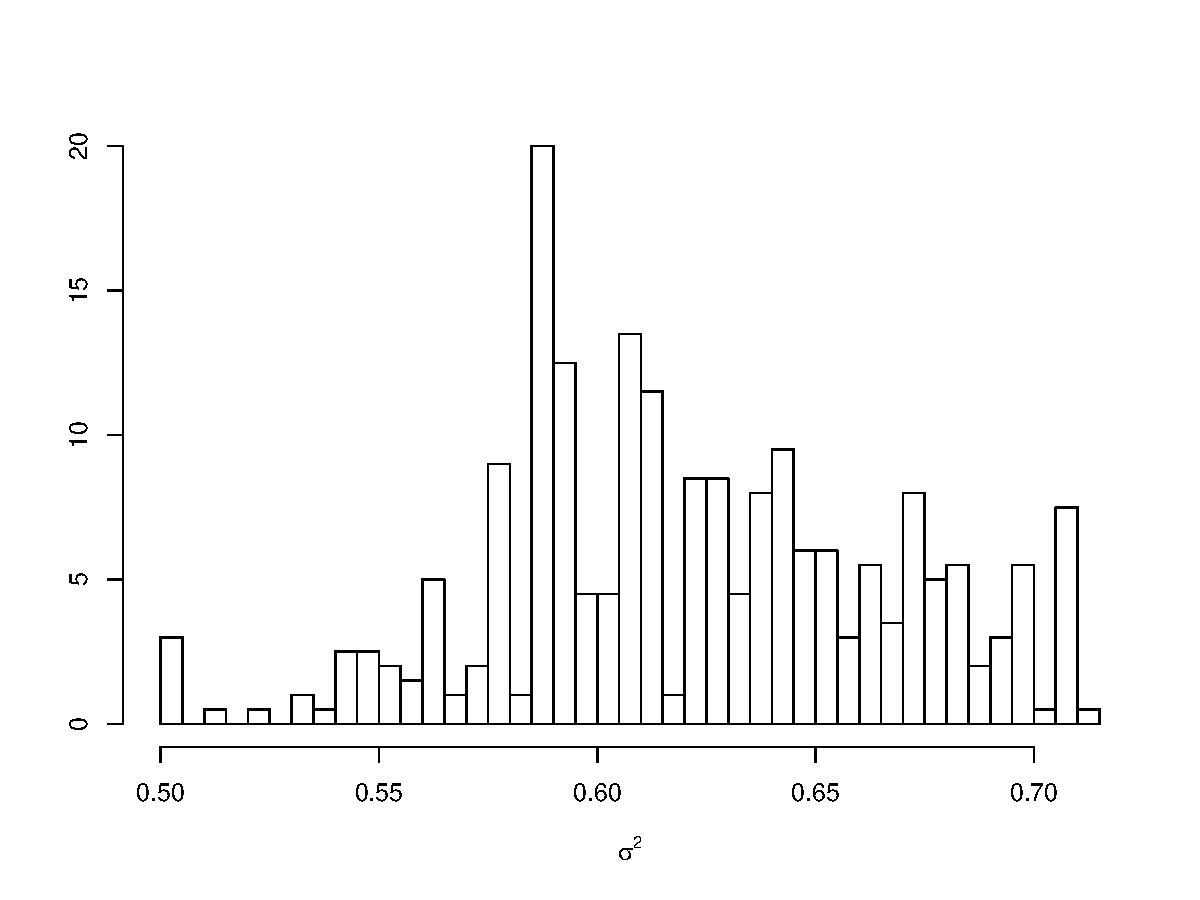
\includegraphics[scale=0.2]{s2_mh_500.pdf}}}%
	\subfloat[Histograma de $\nu$]{{
			\label{fig:nu_mh_500}
			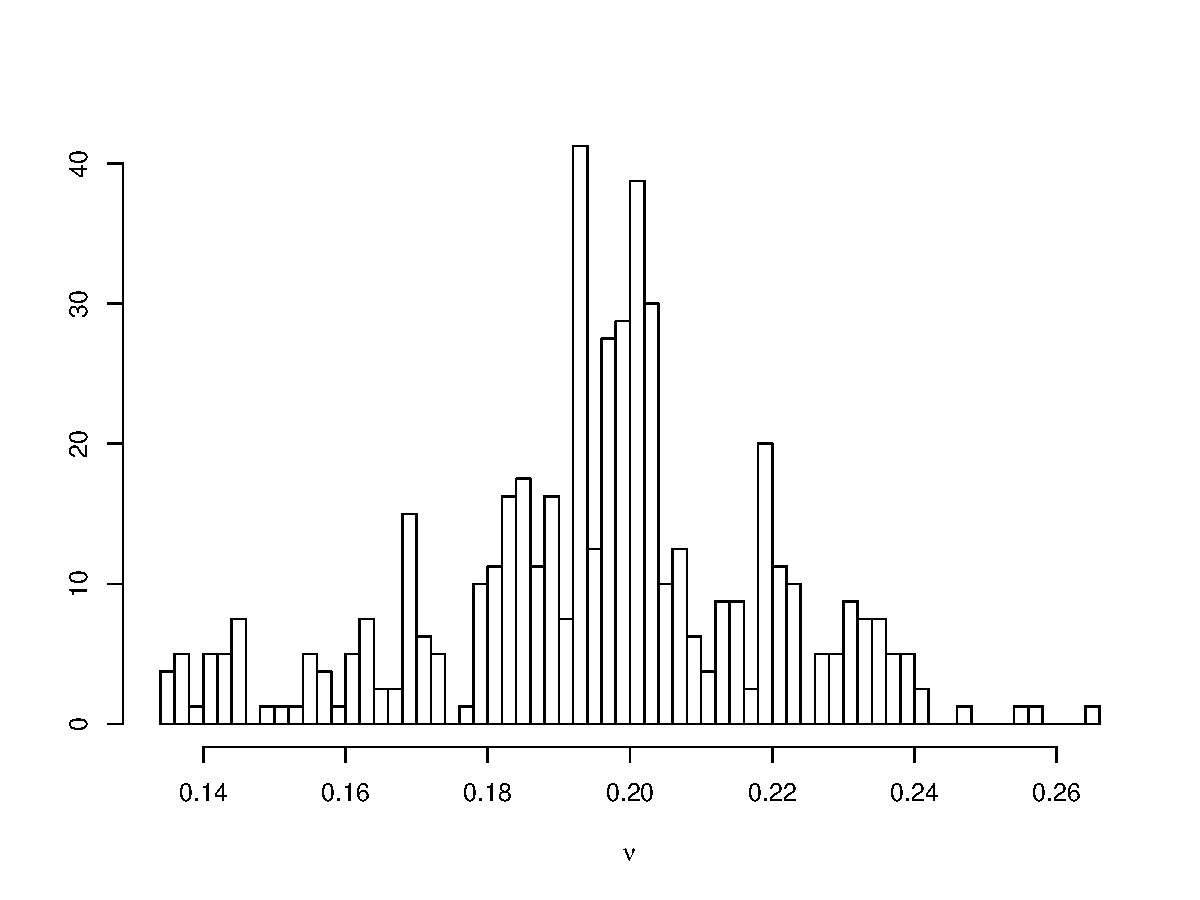
\includegraphics[scale=0.2]{nu_mh_500.pdf}}}%
	\caption{Histograma das densidades \textit{a posteriori} marginais pelo método MCMC--MH, $k = 500$}%
\end{figure}
\end{frame}
% ==================================================
% ==================================================
\begin{frame}
\begin{figure}[t]%
	\centering
	\subfloat[Histograma de $\mu$]{{
			\label{fig:mu_mh_5000}
			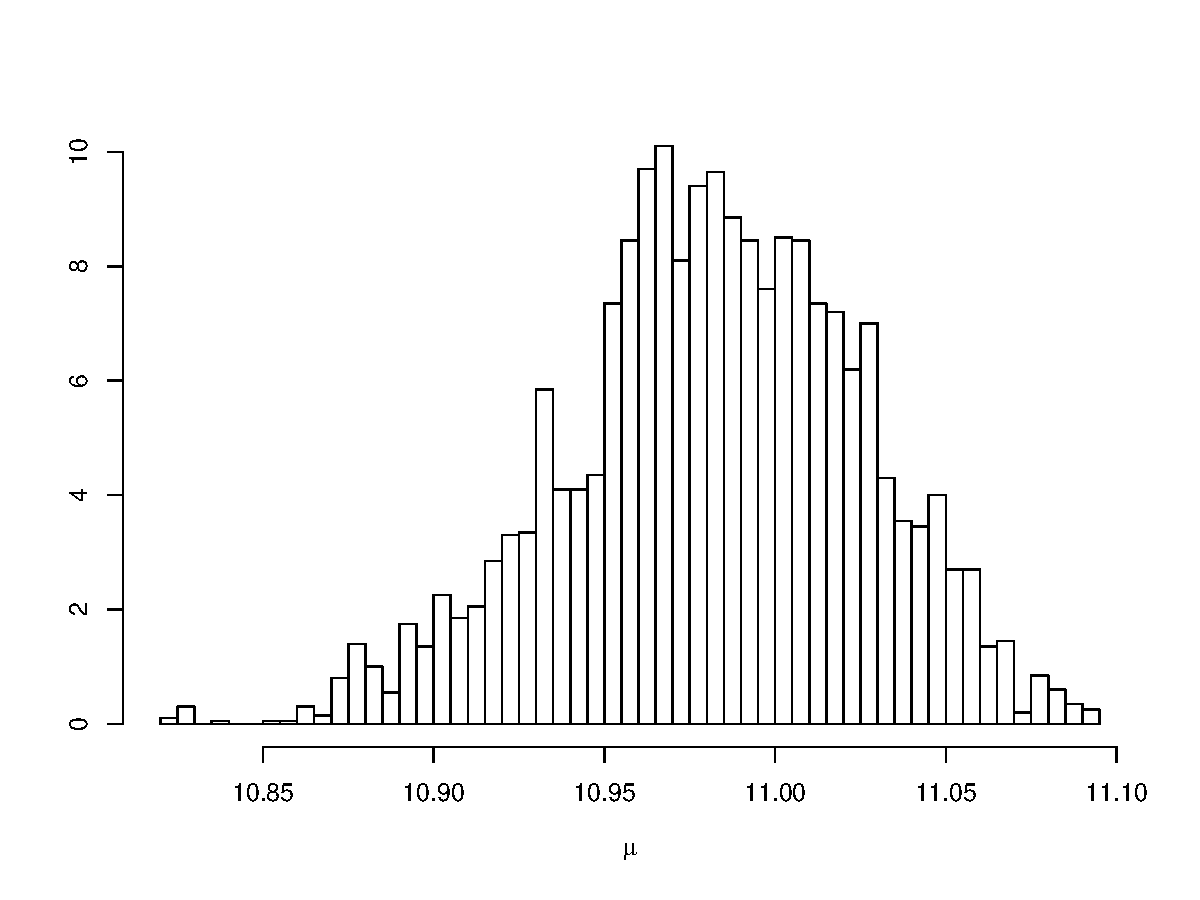
\includegraphics[scale=0.2]{mu_mh_5000.pdf}}}%
	\qquad
	\subfloat[Histograma de $\sigma^2$]{{
			\label{fig:s2_mh_5000}
			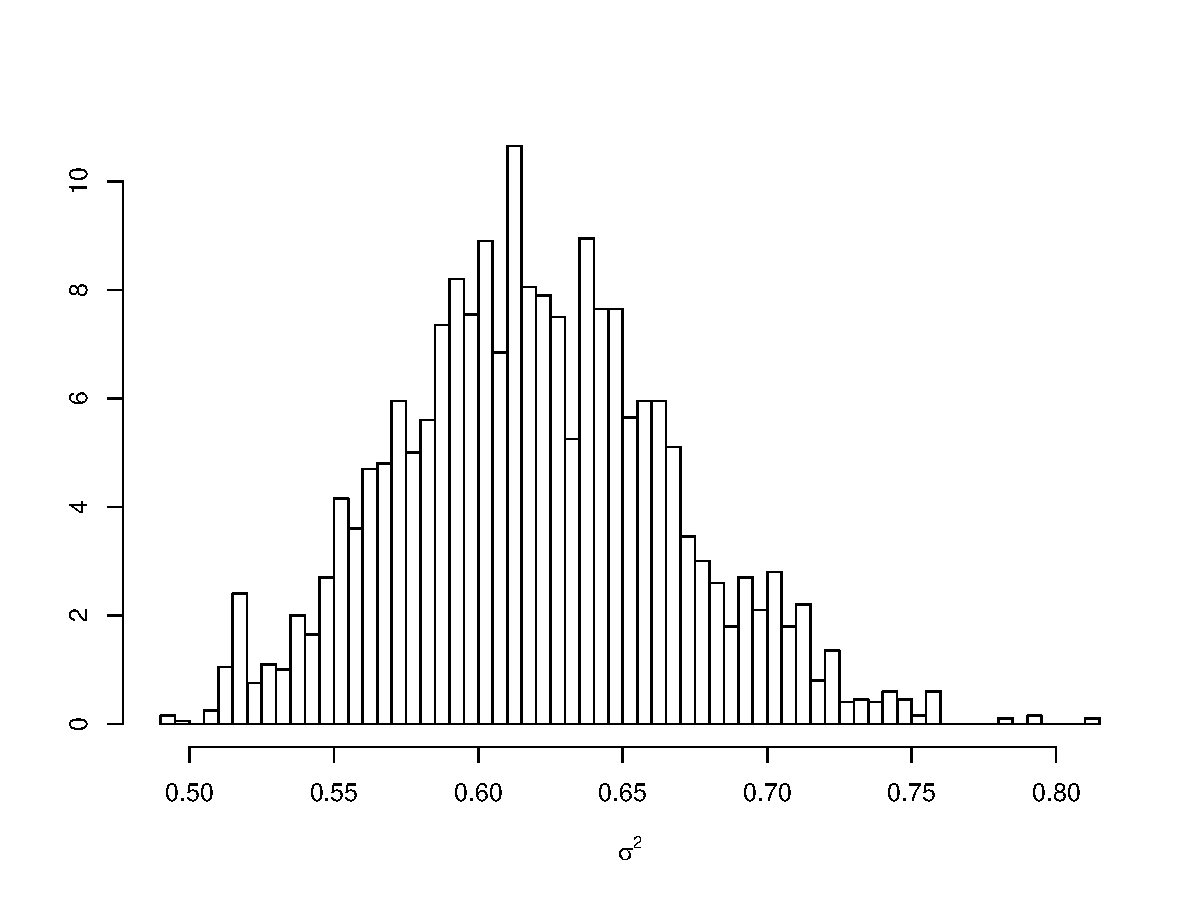
\includegraphics[scale=0.2]{s2_mh_5000.pdf}}}%
	\subfloat[Histograma de $\nu$]{{
			\label{fig:nu_mh_5000}
			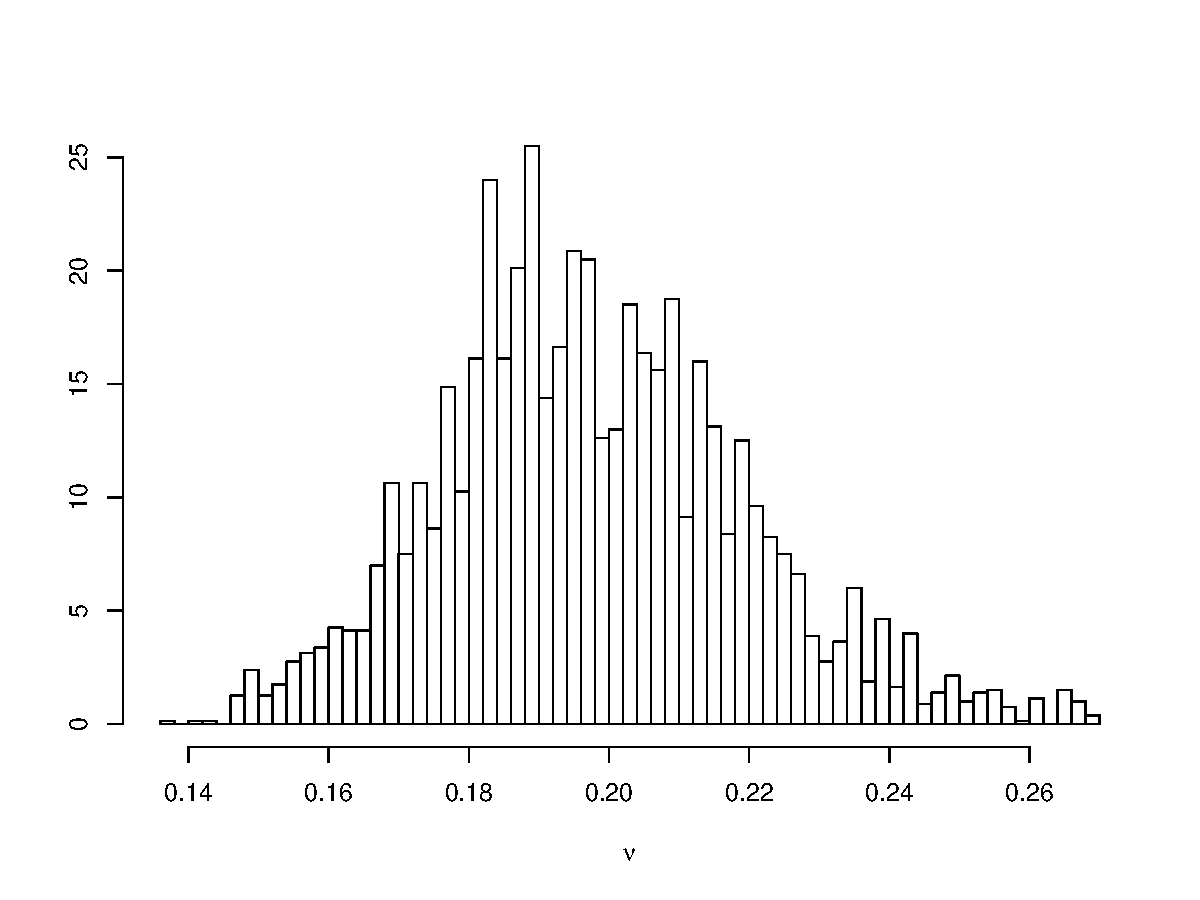
\includegraphics[scale=0.2]{nu_mh_5000.pdf}}}%
	\caption{Histograma das densidades \textit{a posteriori} marginais pela método MCMC--MH, $k = 5000$}%
\end{figure}
\end{frame}
% ==================================================
% ==================================================
\begin{frame}
\begin{figure}[t]%
	\centering
	\subfloat[Histograma de $\mu$]{{
			\label{fig:mu_mh_50000}
			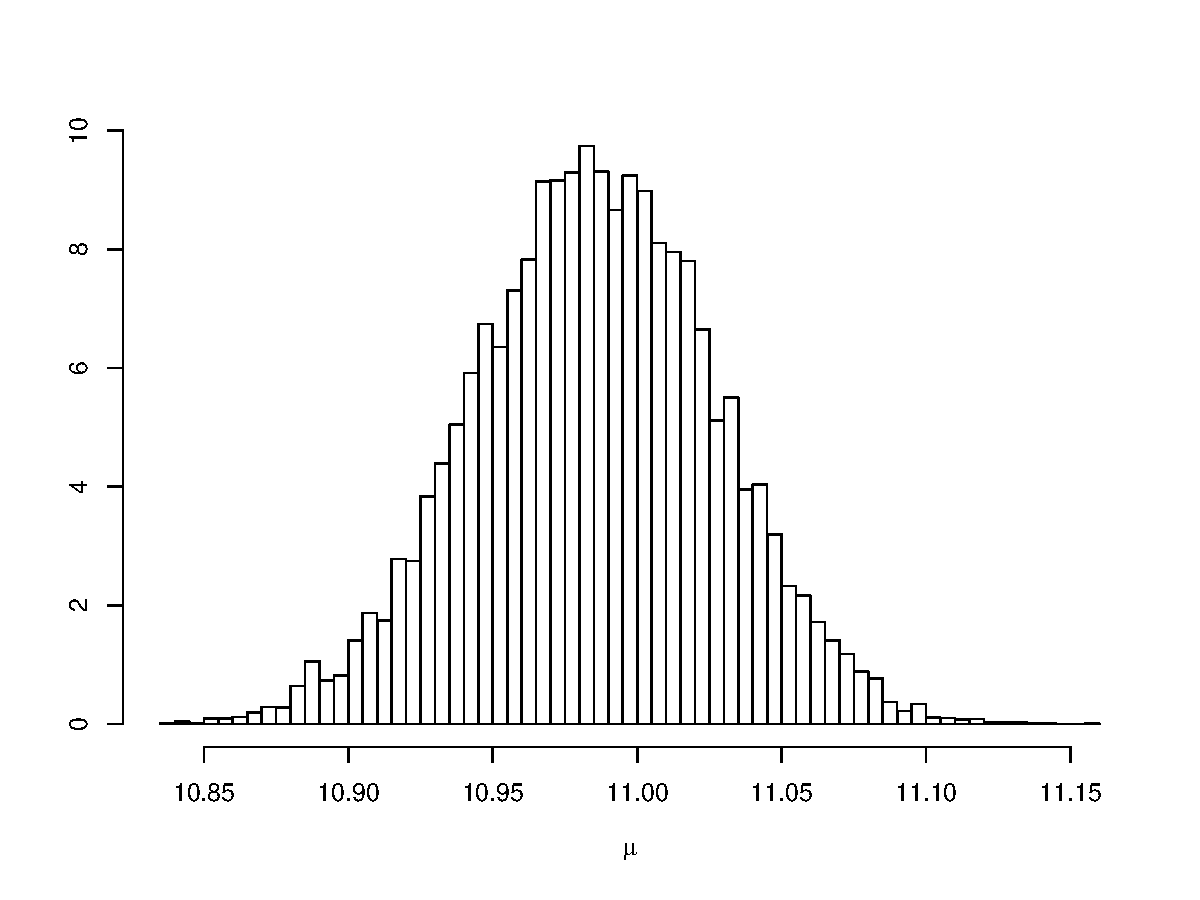
\includegraphics[scale=0.2]{mu_mh_50000.pdf}}}%
	\qquad
	\subfloat[Histograma de $\sigma^2$]{{
			\label{fig:s2_mh_50000}
			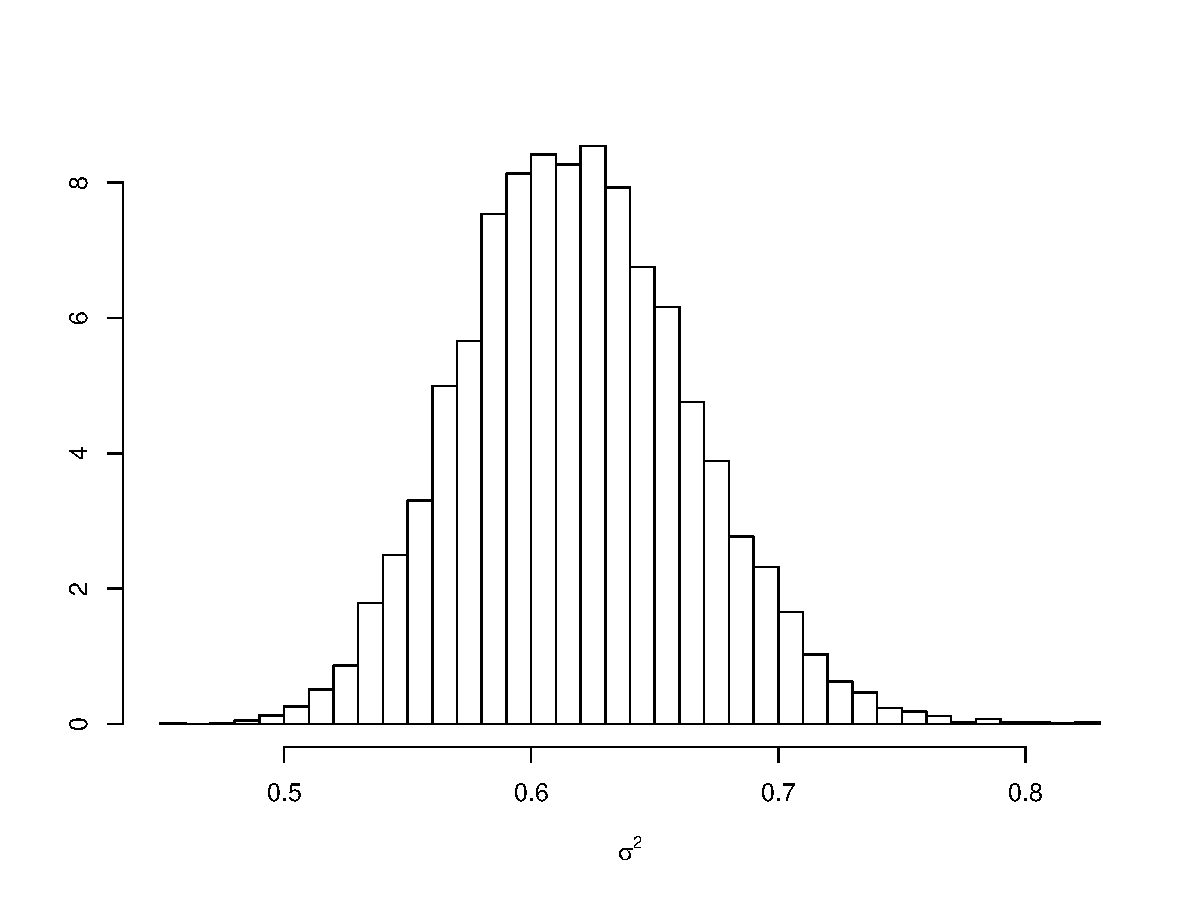
\includegraphics[scale=0.2]{s2_mh_50000.pdf}}}%
	\subfloat[Histograma de $\nu$]{{
			\label{fig:nu_mh_50000}
			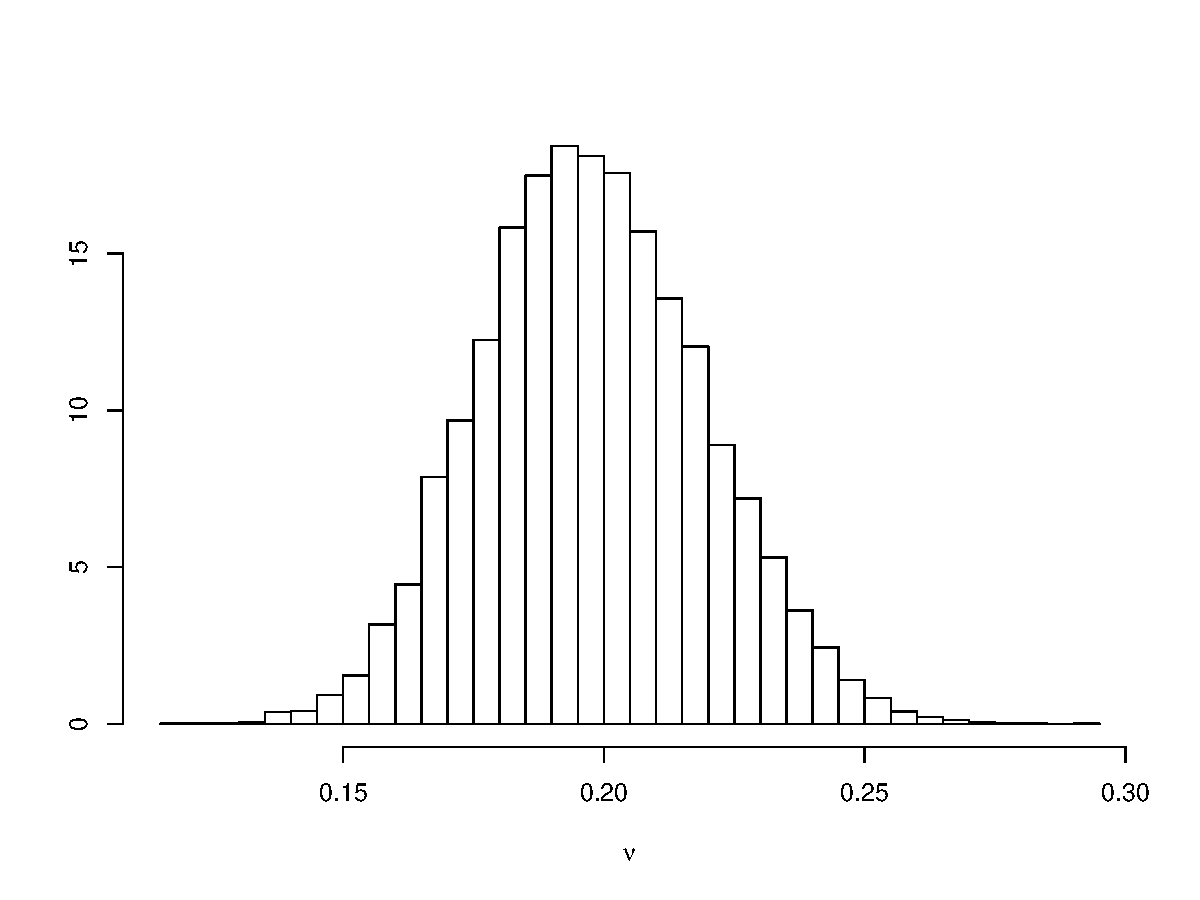
\includegraphics[scale=0.2]{nu_mh_50000.pdf}}}%
	\caption{Histograma das densidades \textit{a posteriori} marginais pela método MCMC--MH, $k = 50000$}%
\end{figure}
\end{frame}
% ==================================================
% ==================================================
\begin{frame}
\begin{table}[htb]
	\caption{Estatísticas \textit{a posteriori} para $(\mu, \sigma^2, \nu)$ pelo método MCMC--MH}
	\label{tab3}
	\centering
	\begin{tabular}{cccccc}
		\toprule
		Cenário & Parâmetro & Média & Variância & Assimetria & Curtose \\
		\midrule
		$k = 500$ & $\mu$ & 10.9672 & 0.0018 & -0.3768 & 3.2193 \\
		& $\sigma^2$ & 0.6226 & 0.0020 & -0.0684 & 2.6117 \\
		& $\nu$      & 0.1957 & 0.0006 & -0.3313 & 3.2991 \\
		\midrule
		$k = 5000$ & $\mu$ & 10.9818 & 0.0019 & -0.2466 & 2.9894 \\
		& $\sigma^2$ & 0.6197 & 0.0023 & 0.2372 & 3.0057 \\
		& $\nu$      & 0.1977 & 0.0005 & 0.3878 & 3.2038 \\
		\midrule
		$k = 50000$ & $\mu$ & 10.9852 & 0.0017 & -0.0272 & 2.9451 \\
		& $\sigma^2$ & 0.6188 & 0.0021 & 0.2472 & 3.1088 \\
		& $\nu$      & 0.1978 & 0.0005 & 0.1331 & 2.8971 \\
		\bottomrule
	\end{tabular}
\end{table}
\end{frame}
% ==================================================
% ==================================================
\begin{frame}
\begin{figure}[htb]
	\centering
	\subfloat[Traço de $\mu$]{{
			\label{fig:trace_mu_mh}
			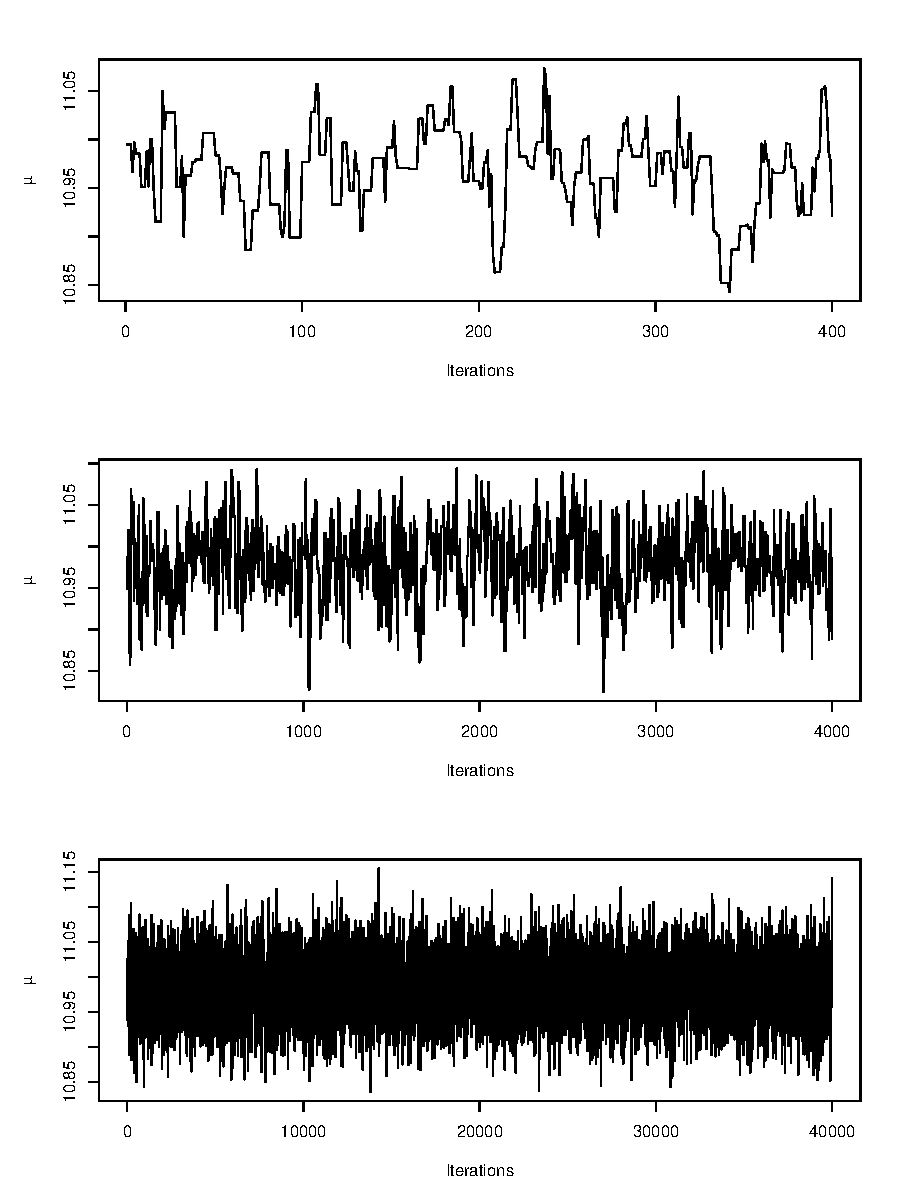
\includegraphics[scale=0.32]{trace_mu_mh.pdf}}}%
	\qquad
	\subfloat[Autocorrelação de $\mu$]{{
			\label{fig:acf_mu_mh}
			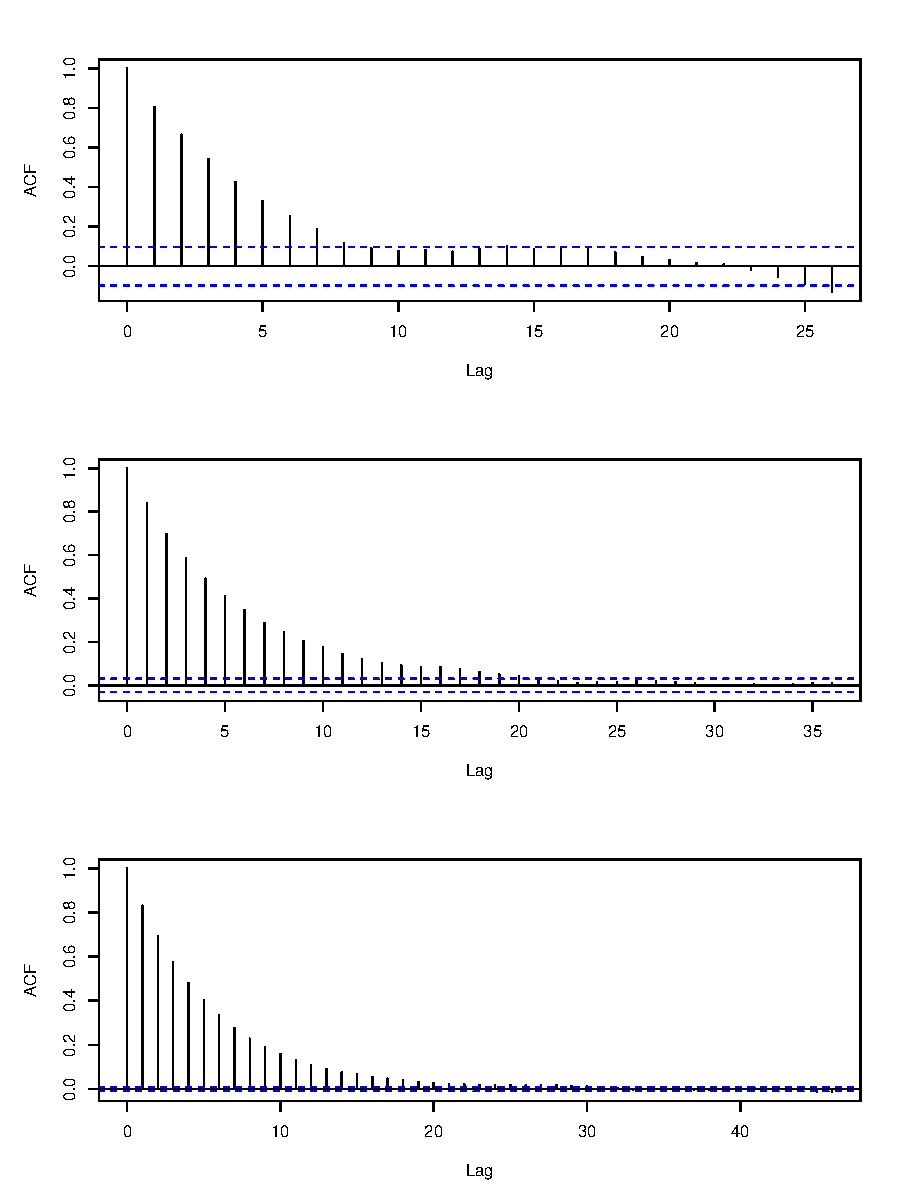
\includegraphics[scale=0.32]{acf_mu_mh.pdf}}}%
	\caption{Traço e autocorrelação da cadeia de $\mu$, $k = \{500, 5000, 50000\}$, respectivamente}%
\end{figure}
\end{frame}
% ==================================================
% ==================================================
\begin{frame}
\begin{figure}[htb]
	\centering
	\subfloat[Traço de $\sigma^2$]{{
			\label{fig:trace_s2_mh}
			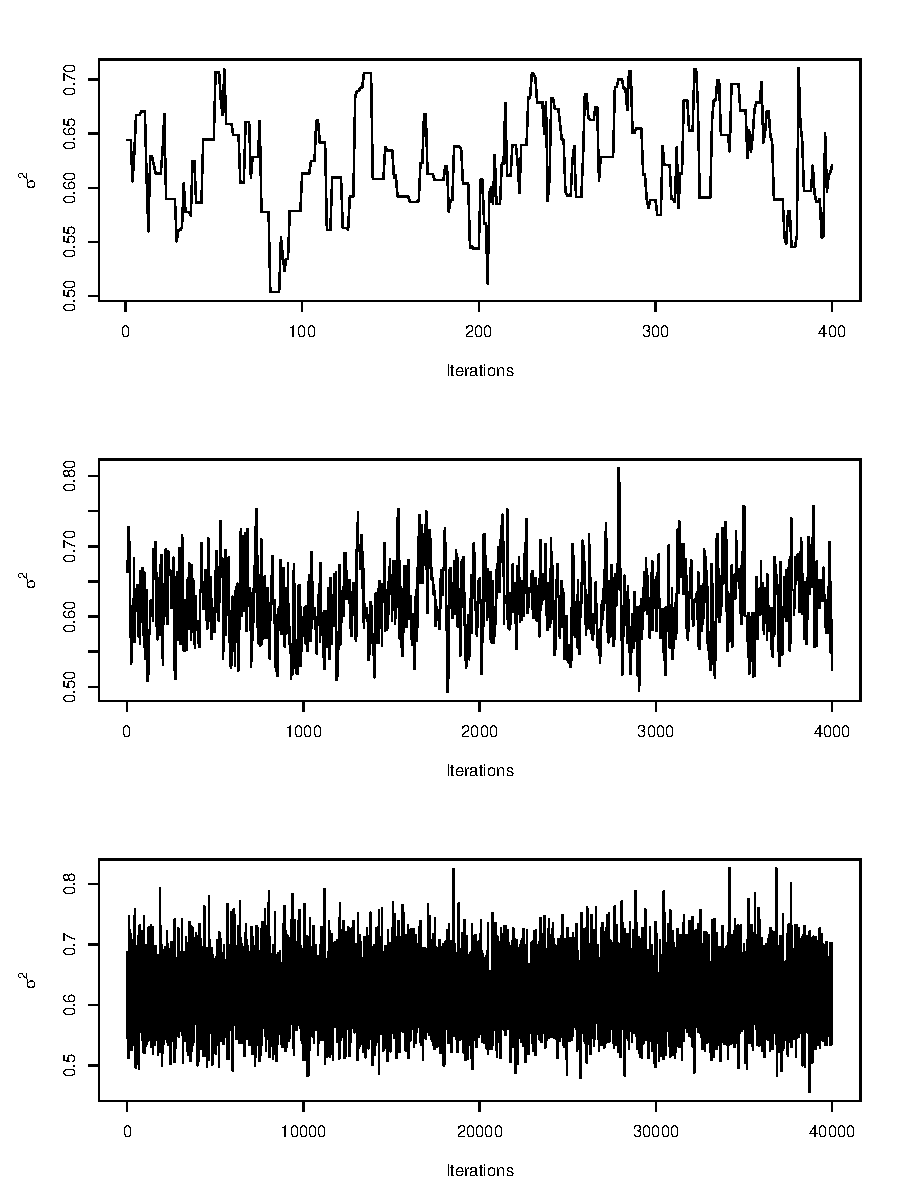
\includegraphics[scale=0.32]{trace_s2_mh.pdf}}}%
	\qquad
	\subfloat[Autocorrelação de $\sigma^2$]{{
			\label{fig:acf_s2_mh}
			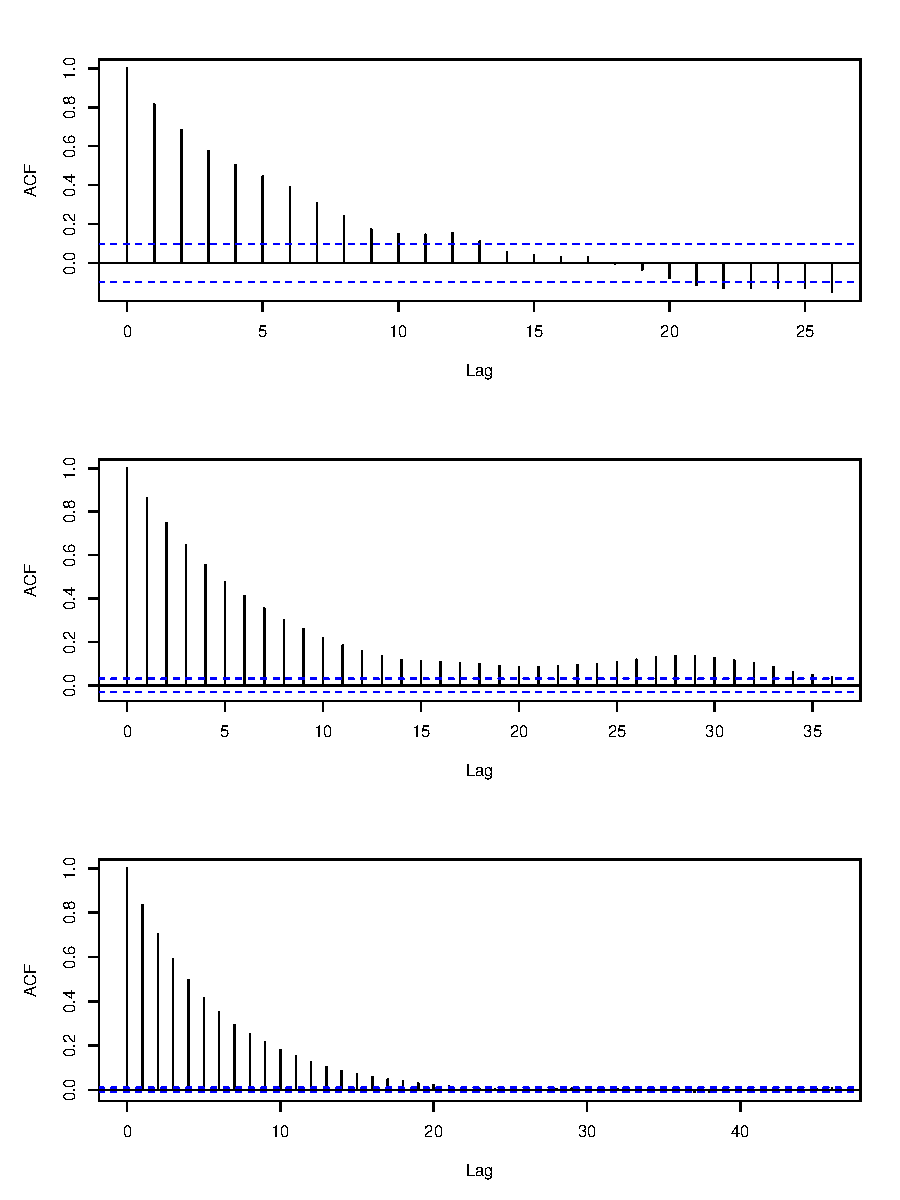
\includegraphics[scale=0.32]{acf_s2_mh.pdf}}}%
	\caption{Traço e autocorrelação da cadeia de $\sigma^2$, $k = \{500, 5000, 50000\}$, respectivamente}%
\end{figure}
\end{frame}
% ==================================================
% ==================================================
\begin{frame}
\begin{figure}[htb]
	\centering
	\subfloat[Traço de $\nu$]{{
			\label{fig:trace_nu_mh}
			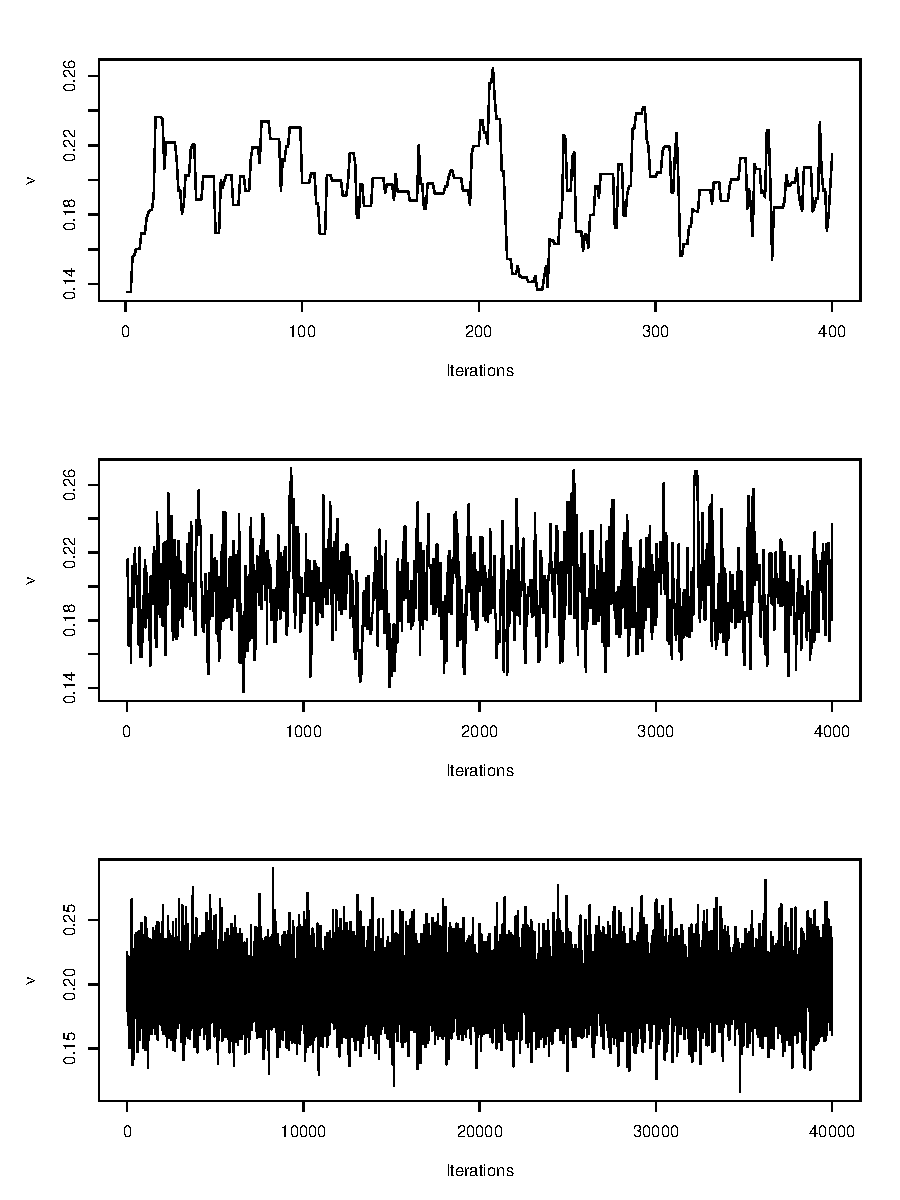
\includegraphics[scale=0.32]{trace_nu_mh.pdf}}}%
	\qquad
	\subfloat[Autocorrelação de $\nu^2$]{{
			\label{fig:acf_nu_mh}
			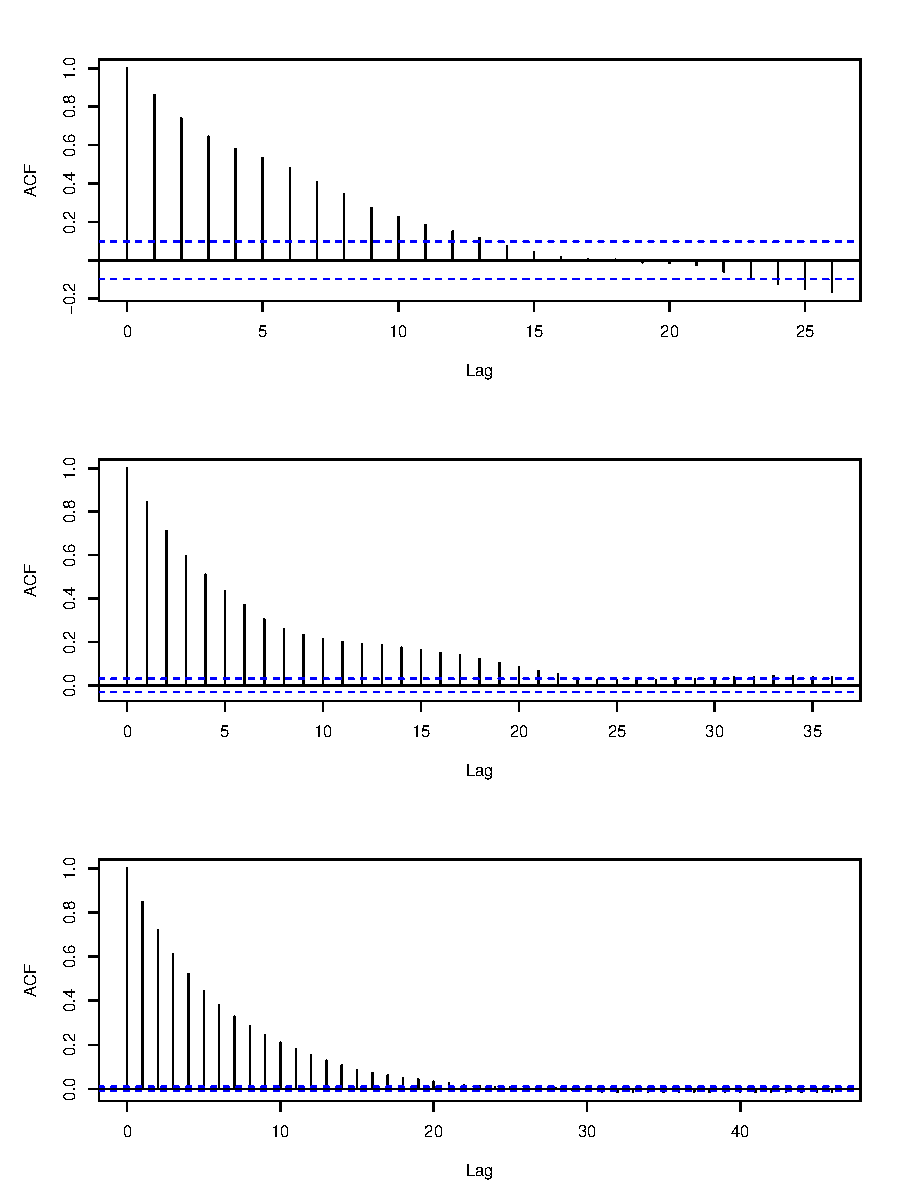
\includegraphics[scale=0.32]{acf_nu_mh.pdf}}}%
	\caption{Traço e autocorrelação da cadeia de $\nu^2$, $k = \{500, 5000, 50000\}$, respectivamente}%
\end{figure}
\end{frame}
% ==================================================
% ==================================================
\section{Considerações finais}
\begin{frame}
\end{frame}

%\section{Referências}
%\begin{frame}[allowframebreaks]
%\frametitle{Referências}
%\justifying 
%Berkson, J., Gage, R.P., (1952). Survival cure for cancer patients following treatment. \textit{Journal of the American Statistical Association}.
%\end{frame}	

\end{document}